%% This is the ctufit-thesis example file. It is used to produce theses
%% for submission to Czech Technical University, Faculty of Information Technology.
%%
%% Get the newest version from
%% https://gitlab.fit.cvut.cz/theses-templates/FITthesis-LaTeX
%%
%%
%% Copyright 2021, Eliska Sestakova and Ondrej Guth
%%
%% This work may be distributed and/or modified under the
%% conditions of the LaTeX Project Public Licenese, either version 1.3
%% of this license or (at your option) any later version.
%% The latest version of this license is in
%%  https://www.latex-project.org/lppl.txt
%% and version 1.3 or later is part of all distributions of LaTeX
%% version 2005/12/01 or later.
%%
%% This work has the LPPL maintenance status `maintained'.
%%
%% The current maintainer of this work is Ondrej Guth.
%% Contact ondrej.guth@fit.cvut.cz for bug reports.
%% Alternatively, submit bug reports into the tracker at
%% https://gitlab.fit.cvut.cz/theses-templates/FITthesis-LaTeX/issues
%%
%%

%%%%%%%%%%%%%%%%%%%%%%%%%%%%%%%%%%%%%%%%%
% CLASS OPTIONS
% language: czech/english/slovak
% thesis type: bachelor/master/dissertation
%%%%%%%%%%%%%%%%%%%%%%%%%%%%%%%%%%%%%%%%%
\documentclass[czech,bachelor,unicode]{ctufit-thesis}

%%%%%%%%%%%%%%%%%%%%%%%%%%%%%%%%%%
% FILL IN THIS INFORMATION
%%%%%%%%%%%%%%%%%%%%%%%%%%%%%%%%%%
\ctufittitle{Webová aplikace pro sledování vývoje cen kryptoměn} % replace with the title of your thesis
\ctufitauthorfull{Jan Koten} % replace with your full name (first name(s) and then family name(s) / surname(s)) including academic degrees
\ctufitauthorsurnames{Koten} % replace with your surname(s) / family name(s)
\ctufitauthorgivennames{Jan} % replace with your first name(s) / given name(s)
\ctufitsupervisor{Ing. Stanislav Kuznetsov} % replace with name of your supervisor/advisor (include academic degrees)
\ctufitdepartment{Katedra aplikované matematiky} % replace with the department of your defence
\ctufityear{2022} % replace with the year of your defence
\ctufitdeclarationplace{Praze} % replace with the place where you sign the declaration
\ctufitdeclarationdate{\today} % replace with the date of signature of the declaration
\ctufitabstractCZE{Tato práce se zabývá problematikou predikce vývoje hodnoty kryptoměn. V rámci ní je vytvořena webová aplikace poskytující uživatelům informace, jako jsou počátek, konec a hodnota následujících lokálních extrémů. Tyto údaje jsou aplikací predikovány v rámci desítek minut do budoucnosti. Společně s historickou hodnotou kryptoměn jsou zaznamenávána data o vyhledávání dané kryptoměny v čase na vyhledávači Google a~data o vývoji hodnot VIX, S\&P 500 a zlata. Predikce aplikace jsou uskutečněny právě na základě těchto dat. Zároveň jsou zaznamenaná data zobrazována v aplikaci ve formě grafu. Uživatelům je pak v reálném čase poskytováno doporučení o akcích, které mají provést pro zajištění výdělku. Těmito akcemi jsou prodej, nákup a nečinnost v rámci jednotlivých kryptoměn. Takto je aplikace schopná pomoci uživatelům ve zlepšení orientace na trhu s kryptoměnami.}
%
\ctufitabstractENG{This work deals with the issue of predicting the development of cryptocurrency. Within it, a~web application is created that provides users with information such as the beginning, end and value of the following local extremes. This data is predicted by the application within tens of minutes into the future. Along with the historical value of cryptocurrencies, we are also recording searches of cryptocurrencies on Google and data from the development of VIX, S\&P 500 and gold values. Application predictions are made on the basis of this data. At the same time, the recorded data is displayed in the application in the form of a graph. Users are then provided with real-time recommendations on the actions they need to take to earn money. These actions are sales, purchases and inactivity within individual cryptocurrencies. In this way, the application is able to help users improve their orientation in the cryptocurrency market.}
\ctufitkeywordsCZE{predikce hodnoty kryptoměn, umělá inteligence, webová aplikace, scraping webu, nestandardní ukazatele, Python, TensorFlow, Vue.js}
\ctufitkeywordsENG{cryptocurrency value prediction, artificial inteligence, web application, web scraping, nonstandard indicators, Python, TensorFlow, Vue.js}
%%%%%%%%%%%%%%%%%%%%%%%%%%%%%%%%%%
% END FILL IN
%%%%%%%%%%%%%%%%%%%%%%%%%%%%%%%%%%

%%%%%%%%%%%%%%%%%%%%%%%%%%%%%%%%%%
% CUSTOMIZATION of this template
% Skip this part or alter it if you know what you are doing.
%%%%%%%%%%%%%%%%%%%%%%%%%%%%%%%%%%

\RequirePackage{iftex}[2020/03/06]
\iftutex % XeLaTeX and LuaLaTeX
    \RequirePackage{ellipsis}[2020/05/22] %ellipsis workaround for XeLaTeX
\else
    \RequirePackage[utf8]{inputenc}[2018/08/11] %this file encoding
    \RequirePackage{lmodern}[2009/10/30] % vector flavor of Computer Modern font
\fi

% hyperlinks
\RequirePackage[pdfpagelayout=TwoPageRight,colorlinks=false,allcolors=decoration,pdfborder={0 0 0.1}]{hyperref}[2020-05-15]

% uncomment the following to hide all hyperlinks
% \RequirePackage[pdfpagelayout=TwoPageRight,hidelinks]{hyperref}[2020-05-15]

\RequirePackage{pdfpages}[2020/01/28]

\setcounter{secnumdepth}{4} % numbering sections; 4: subsubsection



%%%%%%%%%%%%%%%%%%%%%%%%%%%%%%%%%%
% CUSTOMIZATION of this template END
%%%%%%%%%%%%%%%%%%%%%%%%%%%%%%%%%%


%%%%%%%%%%%%%%%%%%%%%%
% DEMO CONTENTS SETTINGS
% You may choose to modify this part.
%%%%%%%%%%%%%%%%%%%%%%
\usepackage{dirtree}
\usepackage{xurl}
\usepackage{lipsum,tikz}
\usepackage{dirtree}
\usepackage{csquotes}
\usepackage[style=iso-numeric]{biblatex}
\usepackage{xcolor}
\addbibresource{text/bib-database.bib}
\usepackage{listings} % typesetting of sources
\usepackage{afterpage}
% \usepackage{minted} % typesetting of sources

%theorems, definitions, etc.
\theoremstyle{plain}
\newtheorem{theorem}{Věta}
\newtheorem{lemma}[theorem]{Tvrzení}
\newtheorem{corollary}[theorem]{Důsledek}
\newtheorem{proposition}[theorem]{Návrh}
\newtheorem{definition}[theorem]{Definice}
\theoremstyle{definition}
\newtheorem{example}[theorem]{Příklad}
\theoremstyle{remark}
\newtheorem{note}[theorem]{Poznámka}
\newtheorem*{note*}{Poznámka}
\newtheorem{remark}[theorem]{Pozorování}
\newtheorem*{remark*}{Pozorování}
\numberwithin{theorem}{chapter}
%theorems, definitions, etc. END
%%%%%%%%%%%%%%%%%%%%%%
% DEMO CONTENTS SETTINGS END
%%%%%%%%%%%%%%%%%%%%%%

\lstdefinelanguage{json}{
    basicstyle=\normalfont\ttfamily,
    numberstyle=\scriptsize,
    stepnumber=1,
    numbersep=8pt,
    showstringspaces=false,
    breaklines=true,
    frame=lines,
    literate=
     *{0}{{{0}}}{1}
      {1}{{{1}}}{1}
      {2}{{{2}}}{1}
      {3}{{{3}}}{1}
      {4}{{{4}}}{1}
      {5}{{{5}}}{1}
      {6}{{{6}}}{1}
      {7}{{{7}}}{1}
      {8}{{{8}}}{1}
      {9}{{{9}}}{1}
      {:}{{{{:}}}}{1}
      {.}{{{{.}}}}{1}
      {,}{{{{,}}}}{1}
      {\{}{{{{\{}}}}{1}
      {\}}{{{{\}}}}}{1}
      {[}{{{{[}}}}{1}
      {]}{{{{]}}}}{1},
}

\begin{document} 
\frontmatter\frontmatterinit % do not remove these two commands

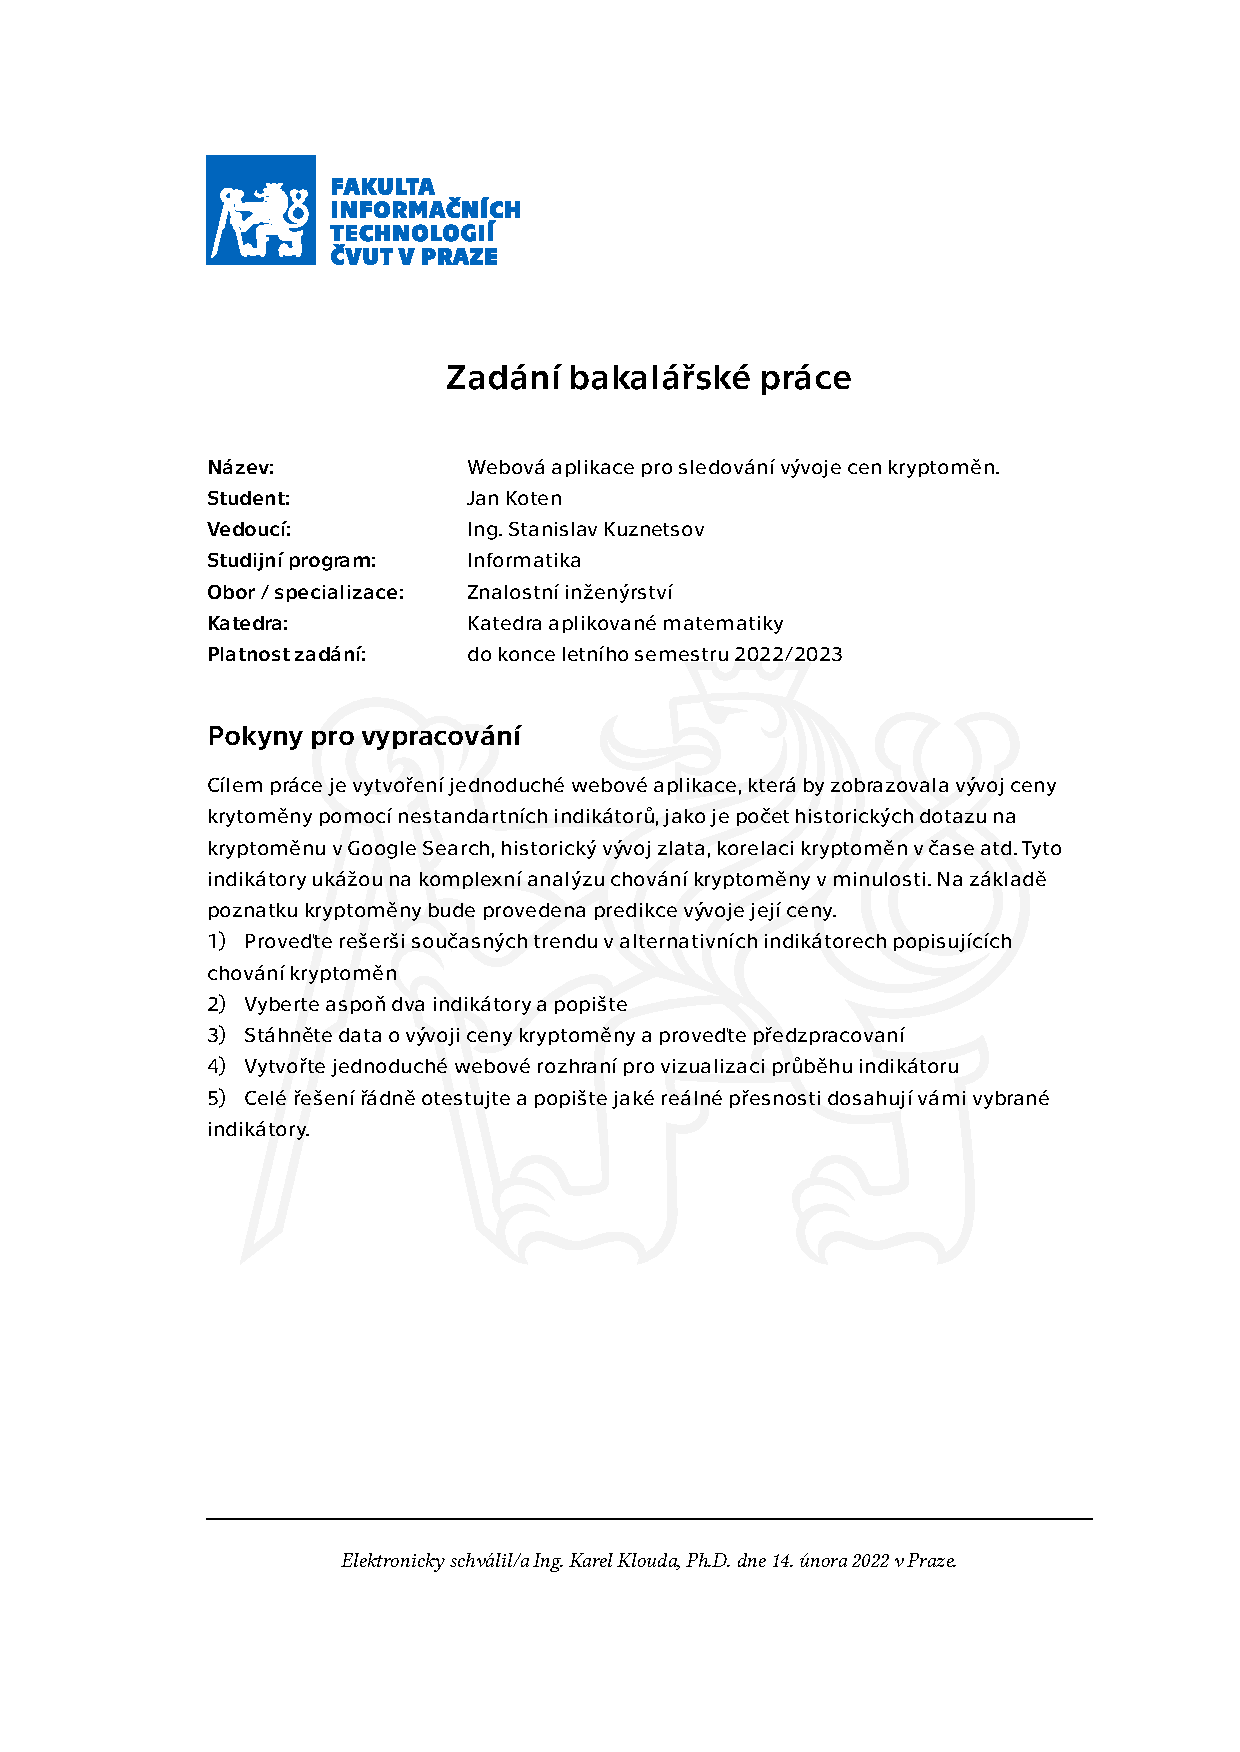
\includepdf{assignment-include.pdf} % replace that file with your thesis assignment provided by study office

\thispagestyle{empty}\cleardoublepage\maketitle % do not remove these three commands

\imprintpage % do not remove this command

\tableofcontents % do not remove this command
%%%%%%%%%%%%%%%%%%%%%%
% list of other contents: figures, tables, code listings, algorithms, etc.
% add/remove commands accordingly
%%%%%%%%%%%%%%%%%%%%%%
\listoffigures % list of figures
\begingroup
\let\clearpage\relax
\listoftables % list of tables
\lstlistoflistings % list of source code listings generated by the listings package
% \listoflistings % list of source code listings generated by the minted package
\endgroup
%%%%%%%%%%%%%%%%%%%%%%
% list of other contents END
%%%%%%%%%%%%%%%%%%%%%%

%%%%%%%%%%%%%%%%%%%
% ACKNOWLEDGMENT
% FILL IN / MODIFY
% This is a place to thank people for helping you. It is common to thank your supervisor.
%%%%%%%%%%%%%%%%%%%

\begin{acknowledgmentpage}
	Chtěl bych poděkovat především vedoucímu své práce Ing. Stanislavu Kuznetsovovi, za jeho vzorové vedení práce a jeho trpělivost. Dále bych pak chtěl poděkovat Milanu Hemžalovi za cenné rady v~průběhu vývoje aplikace a své rodině a přátelům za mentální podporu a pomoc nejen při tvorbě této práce, ale i v průběhu mého studia.
\end{acknowledgmentpage} 
%%%%%%%%%%%%%%%%%%%
% ACKNOWLEDGMENT END
%%%%%%%%%%%%%%%%%%%


%%%%%%%%%%%%%%%%%%%
% DECLARATION
% FILL IN / MODIFY
%%%%%%%%%%%%%%%%%%%
% INSTRUCTIONS
% ENG: choose one of approved texts of the declaration. DO NOT CREATE YOUR OWN. Find the approved texts at https://courses.fit.cvut.cz/SFE/download/index.html#_documents (document Declaration for FT in English)
% CZE/SLO: Vyberte jedno z fakultou schvalenych prohlaseni. NEVKLADEJTE VLASTNI TEXT. Schvalena prohlaseni najdete zde: https://courses.fit.cvut.cz/SZZ/dokumenty/index.html#_dokumenty (prohlášení do ZP)
\begin{declarationpage}
Prohlašuji, že jsem předloženou práci vypracoval samostatně a že jsem uvedl
veškeré použité informační zdroje v souladu s Metodickým pokynem o dodržování etických principů při přípravě vysokoškolských závěrečných prací.
Beru na vědomí, že se na moji práci vztahují práva a povinnosti vyplývající
ze zákona č. 121/2000 Sb., autorského zákona, ve znění pozdějších předpisů.
V souladu s ust. § 2373 odst. 2 zákona č. 89/2012 Sb., občanský zákoník, ve
znění pozdějších předpisů, tímto uděluji nevýhradní oprávnění (licenci) k užití
této mojí práce, a to včetně všech počítačových programů, jež jsou její součástí
či přílohou a veškeré jejich dokumentace (dále souhrnně jen ”
Dílo“), a to všem
osobám, které si přejí Dílo užít. Tyto osoby jsou oprávněny Dílo užít jakýmkoli
způsobem, který nesnižuje hodnotu Díla a za jakýmkoli účelem (včetně užití
k výdělečným účelům). Toto oprávnění je časově, teritoriálně i množstevně
neomezené. Každá osoba, která využije výše uvedenou licenci, se však zavazuje udělit ke každému dílu, které vznikne (byť jen zčásti) na základě Díla,
úpravou Díla, spojením Díla s jiným dílem, zařazením Díla do díla souborného
či zpracováním Díla (včetně překladu) licenci alespoň ve výše uvedeném rozsahu a zároveň zpřístupnit zdrojový kód takového díla alespoň srovnatelným
způsobem a ve srovnatelném rozsahu, jako je zpřístupněn zdrojový kód Díla.
\end{declarationpage}
%%%%%%%%%%%%%%%%%%%
% DECLARATION END
%%%%%%%%%%%%%%%%%%%

\printabstractpage % do not remove this command

\chapter{Seznam zkratek}

\begin{tabular}{rl}
HODL & Hold on for dear life\\
HFT & High frequency trading\\
S\&P 500 & The Standard and Poor's 500\\
ARIMA & Autoregressive integrated moving average\\
RNN & Recurrent neural network\\
ACT/PACF & Autocorrelation and partial autocorrelation function\\
LSTM & Long short term memory\\
GRU & Gated recurrent unit\\
SGD & Stochastic gradient descent\\
RMSProp & Root mean squared propagation\\
GUI & Graphical user interface\\
VPN & Virtual private network\\
HTTP & Hypertext transfer protocol\\
ADF & Augmented Dickey-Fuller test\\
CSS & Cascading Style Sheets\\
HTML & Hypertext markup language\\
API & Application Programming Interface\\
\end{tabular}

\mainmatter\mainmatterinit % do not remove these two commands

%%%%%%%%%%%%%%%%%%%
% THE THESIS
% MODIFY ANYTHING BELOW THIS LINE
%%%%%%%%%%%%%%%%%%%

\chapter*{Úvod}\addcontentsline{toc}{chapter}{Úvod}\markboth{Úvod}{Úvod}
Kryptoměna je digitální forma měny.
Jedná se o prostředek směny využívaný v online světě a její největší předností je decentralizovanost.
Není regulovaná ani udržována žádnou centrální autoritou, jako jsou například vládní orgány nebo banky.
Záznamy o vlastnictví a transakcích s kryptoměnami jsou uloženy v distribuovaných databázích.
Typicky se jedná o využití technologie blockchain. 
Kryptoměny jsou kryptograficky chráněny a pro validaci používají metody jako proof-of-stake, při kterých se ověří platnost historie všech transakcí. 
Validace transakcí kryptoměn je zajištěna blockchainem, tedy neustále rostoucím seznamem navzájem propojených záznamů. 
Každý ze záznamů transakcí obsahuje hash odkazující se na předchozí záznam. 
Tímto způsobem se stávají odolné vůči neoprávněné modifikaci dat. Během posledních let se začalo rozšiřovat povědomí o kryptoměnách prostřednictvím internetu i mimo něj.
Umožňují způsob, jak obejít pokles hodnoty oficiální státní měny a zároveň poskytuje uživatelům lepší formu anonymity při provádění transakcí.
Nejen Bitcoin, jakožto první veřejně známá kryptoměna totiž od svého vzniku výrazně získal na své hodnotě. 
Stejně tak postupně získávaly na hodnotě i~ostatní kryptoměny. 
Od jejich vzniku počínaje kryptoměnou Bitcoin v roce 2009 se jedinci, komunity i~společnosti snažili jejich prostřednictvím finančně obohatit. 
Růst jejich hodnoty měl vliv na vznik mnoha národních i nadnárodních společnosti, z nichž mnoho kapitalizovalo právě na vývoji hodnoty kryptoměn. 
Začaly vznikat kryptoměnové burzy, které nabízely uživatelům velice efektivní způsob obchodování a změny hodnoty jejich konta \cite{cryptodef:1, cryptodef:2}.

Vstup na finanční trh může být pro mnohé nové obchodníky skličující zkušenost. 
Investování do vybraných asetů se nám nemusí vždy vyplatit. 
Pro dosažení výdělku při obchodování s kryptoměnami, je nutné správně odhadnout trend, kterým se daná kryptoměna ubírá. 
Tuto informaci můžeme odhadnout z pouhého sledování dlouhodobého trendu kryptoměny. 
Pro dosažení nejoptimálnějších výsledků však potřebujeme využít co nejvíce zdrojů, které mají prokazatelně vliv na vývoj hodnoty. 
Přístup k této problematice rozhodně není jednotný a existuje tedy mnoho velice odlišných řešení, se kterými se na kryptoměnový trh přistupuje.

Hledání optimálního přístupu k vydělávání na trhu s kryptoměnami je předmětem řešení této práce. 
Na základě analýzy trhu a současných řešení vytvoříme systém, který nám bude schopný poskytovat informace maximalizující naší šanci na výdělek.
Výsledek a také důvod našeho snažení by pak měla být aplikace, která bude pro své uživatele zdrojem konstantního příjmu.

V následných kapitolách budeme analyzovat technologie využívané v současné době na finančním trhu. 
Nebude se jednat o postupy používané pouze při obchodování s kryptoměnami.
Budeme se soustředit zpravidla na přístupy, které mají v našem poli zájmu potenciál využití.
Následně budeme analyzovat technologie a metody, které v naší aplikaci využijeme v závislosti na jejích požadavcích na funkcionality, hardware a software.
Jednotlivě budeme konstruovat systémy pro získávání dat z internetu, zpracování, predikci a zobrazování dat a po ukončení vývoje jednotlivých částí aplikace se budeme věnovat vytváření běhového prostředí pro jejich provoz a~vzájemnou komunikaci.

\chapter*{Cíl práce}\addcontentsline{toc}{chapter}{Cíl práce}\markboth{Cíl práce}{Cíl práce}

Pro obchodování na trhu s kryptoměnami neexistuje žádný jednoznačný přístup, který by nám mohl garantovat výdělek.
Tato skutečnost pro nás znamená, že se na základě prozkoumání současných dostupných řešení můžeme pokusit o konstrukci našeho vlastního. 
Cílem naší práce je vytvoření přehledné webové aplikace, která by zobrazovala vývoj ceny kryptoměn pomocí nestandartních indikátorů, jako je například počet historických dotazu na kryptoměnu v Google Search, historický vývoj zlata nebo korelace kryptoměn v čase.
Tyto indikátory ukážou na komplexní analýzu chování kryptoměny v minulosti.
Dále budou prostřednictvím grafické části aplikace poskytovány vhodné rady ve smyslu nákupu, prodání a nečinnosti v rámci jednotlivých kryptoměn.
Na základě získaných dat o sledovaných kryptoměnách bude provedena predikce vývoje jejich cen.
Budeme provádět rešerši současných trendů v alternativních indikátorech popisujících chování kryptoměn.

V rámci naší aplikace budeme také aktivně a periodicky získávat informace pro predikci z~námi zvolených internetových zdrojů.
Tyto informace budou po vhodném zpracování poskytovány uživateli v rámci webového grafického uživatelského rozhraní.
Jejich poskytování bude realizováno v reálném čase nebo téměř reálném čase se zpožděním a periodou obnovy zobrazení nových informací maximálně v jednotkách minut. 
Data budeme ukládat do databázového systému. Aplikací budou dále zpracována do podoby, ve které z nich bude uskutečněna predikce natrénovaným predikčním modelem. 
Především bude kladen důraz na zobrazování relevantních informací v dostatečně přehledném měřítku a také na jejich přesnost. 
Informace signalizující, že by měl uživatel ihned nakoupit nebo prodat kryptoměnu by měly vést k výdělku pro libovolně zvolenou kryptoměnu.
Lze tedy počítat s tím, že nebude vybrána strategie, která by dosahovala nejlepšího výsledku napříč testovanými daty, ale ta, která bude dosahovat kladného zisku napříč všemi testovanými kryptoměnami.

Při konstrukci aplikace bude nezbytné přizpůsobit vývoj požadavkům na její funkce a užití.
Bude třeba řešit běhové prostředí s ohledem na rychlost a přehlednost.
Rozhodování o jednotlivých akcích doporučených uživatelům bude realizováno na základě predikcí vyhodnocených zvoleným predikčním modelem.
Na základě této predikce bude ke každé uživatelem specifikované kryptoměně možné učinit informovaný odhad vývoje její hodnoty. 
Uživatel pak bude schopný uskutečňovat transakce, které mu budou dlouhodobě přinášet zisk.

V první kapitole zhodnotíme současné postupy při obchodování s kryptoměnami i obecně na finančním trhu. Ve druhé vybereme vhodné nástroje, které nám umožní vývoj aplikace. Dále budeme v jednotlivých kapitolách řešit stahování dat z internetu, predikce vývoje hodnot kryptoměn a zobrazování výsledků prostřednictvím webové aplikace. V poslední kapitole se pak budeme věnovat způsobu zapojení a komunikaci jednotlivých částí aplikace v rámci jednoho celku.

\chapter{Současné přístupy k problematice obchodování s kryptoměnami}

Obchodování s kryptoměnami není zpravidla interpretováno jako forma jednoznačného výdělku. 
Lze ovšem nalézt výjimky v tomto tvrzení.
Tím bývají jedinci, kteří byli schopni, ať už cíleně nebo náhodou, zakoupit kryptoměnu před jejím náhlým zvýšením její hodnoty a zajistit si takto nemalý výdělek. 
Většinu času nelze pouze spoléhat na šťastnou náhodu a je třeba využít patřičných postupů, které zvýší šanci na zisk z našeho obchodování.

V této kapitole se seznámíme se současnými technologiemi používanými při obchodování na trhu s kryptoměnami, ale také s přístupy na ostatních trzích.
Těmi budou například trhy akciové nebo se směnou cizích měn.
Budeme se snažit analyzovat co nejvíce rozdílných přístupů, abychom mohli snáze určit náš vlastní způsob řešení, který bude stavět na úspěších zkoumaných prací.

Vývoj kryptoměn je velice nestálý. 
Hodnota je ovlivněna podílem měny, která se nachází v~oběhu a částkou, kterou je za ní nakupující strana ochotná zaplatit. 
Jedná se tedy o vliv nabídky a poptávky, ale také o sentiment uživatelů a investorů, vládní nařízení či regulace a~mediální informace. 
Mnoho měn včetně Bitcoinu má konečný počet mincí, které budou kdy vydány. 
Můžeme očekávat, že čím blíže se počet mincí kryptoměn bude blížit ke svému konečnému počtu, tím bude jejich hodnota stoupat \cite{volatile}.

Na základě této skutečnosti se ukazuje nemožné nalézt jednotný způsob, který by nám spolehlivě zaručil vysoký výnos. 
Jednotlivé přístupy se často velice liší. 
Základní myšlenka však vždy zůstává stejná. 
Je třeba nakoupit kryptoměnu za menší cenu, než za kterou jí prodáme, abychom na ní mohli vydělat. 
Je také možné nalézt rozdílné kurzy kryptoměn mezi jednotlivými burzami a~tedy transakcemi mezi nimi dosáhnout zisku. 
Proto se postupy při obchodování mohou odvíjet od společných základních principů, u kterých je obecně možné za specifických podmínek dosáhnout zisku. 
Nejpoužívanější z nich jsou HODL, HFT a Obchodování na základě predikce.

\section{HODL}

HODL je pojem odvozený od překlepu anglického slova \uv{hold}. 
Jedná se o strategii, při které uživatel zakoupí kryptoměnu a dlouhodobě si jí ponechá bez ohledu na její současnou hodnotu. 
Prodej nastává pouze ve chvíli, kdy se její hodnota značně odchýlí od její kupní ceny. 
Tento dlouhodobý přístup je volen zejména ve chvíli, kdy se uživatelé chtějí co nejvíce oprostit od aktivního sledování vývoje ceny kryptoměny. 
Je volen zejména jedinci bez předchozích zkušeností s obchodováním kvůli jejich sníženým schopnostem správně načasovat výhodnou koupi nebo prodej.  
V tomto způsobu obchodování nefigurují žádné algoritmy nebo predikční modely a jedná se o~nejjednodušší formu obchodování. 
Zároveň ale ne o nejvýnosnější \cite{hodl}.

\section{HFT}

Vysokofrekvenční obchodování je metoda obchodování, která, jak už z názvu vypovídá, využívá množství příkazů k transakci provedených za sebou i v rozmezí jedné vteřiny. 
Využívá analýzy mnoha různých trhů a kryptoměnových burz. 
Při tomto typu obchodování platí, že obchodníci s~vyšší rychlostí a získáváním dat dosahují více ziskových transakcí a celkově jsou tedy úspěšnější, než ti s pomalejším prováděním transakčních operací. 
Pokud algoritmus určený k analýze trhu objeví posloupnost transakcí, která vede k pozitivnímu zisku, neprodleně tuto transakci provede. 

Tento způsob obchodování dodává trhům likviditu a eliminuje malé rozpětí mezi nabídkou a~poptávkou. 
Jedná se o částku, o kterou vyvolávací cena převyšuje nabídkovou cenu kryptoměny na trhu. 
Jinými slovy jde o nejvyšší cenu, kterou je kupující ochoten za kryptoměnu zaplatit a~nejnižší kupní cenou, kterou je prodávající ochoten přijmout. 
Přístup vysokofrekvenčního obchodování začal nabírat na popularitě, když burzy, jako například Newyorská burza cenných papírů, začaly vybízet společnosti, aby na trh přidaly likviditu. 
Ta ve své podstatě udává, jak efektivně lze kryptoměnu, nebo jakékoliv jiné aktivum, či cenný papír směnit za hotovost, aniž by byla ovlivněna původní tržní cena \cite{liquidity}.
Vysokofrekvenční obchodování mělo prokazatelně pozitivní vliv na likviditu trhu a snížilo rozpětí mezi nabídkou~a poptávkou, která se kryptoměn týkala. 
Toto bylo otestováno například ve studii, která zkoumala trh po zavedení poplatků za transakce při vysokofrekvenčním obchodování, což mělo na vydělávání touto metodou negativní vliv. 
Studie zjistila, že tento krok zvýšil rozdíly mezi nabídkou a poptávkou o 13 \% \cite{hft:1, hft:2}.

Vysokofrekvenční obchodování má však svá úskalí, a to především pro jednotlivé obchodníky. 
Tento přístup vyžaduje vysokorychlostní připojení pro rychlý a efektivní zisk informací. 
Je také důležité uvažovat i o čase, který trvá přenesení informace od serveru k uživateli. 
Ten by měl být připojený geograficky co nejblíže k serveru, ze kterého získává informace. 
Samotný přístup k informacím je také velice omezený. 
Poskytování informaci v reálném čase a v dostatečném množství je vždy buď zpoplatněno nebo přinejmenším penalizováno časem před odeslání informace nebo množstvím informací. 
Uživatel dále potřebuje výkonný server pro nalezení vhodných transakcí, které má uskutečnit pro zajištění zisku, a to i v případě, že se rozhodne za poskytování dat platit namísto složitého obcházení omezení od poskytovatelů těchto dat.

Vysokofrekvenční obchodování je často předmětem kritiky. Vysoká rychlost obchodování může být teoreticky schopná způsobit velký a zdánlivě bezdůvodný pohyb na trhu. 
V roce 2010 zažil akciový trh náhlý pokles Dow Jones Industrial Average o 1.5 \%. 
Zpočátku nevysvětlitelný pokles byl předmětem vládního vyšetřování, jehož výsledkem byl nález vysokého množství objednávek, které tento pokles vyvolaly \cite{investigation-hft}.

\section{Predikce}

Nejčastěji využívanou metodou pro obchodování s kryptoměnami je provádění transakcí na základě predikce vývoje hodnoty kryptoměn. 
Obchodník v tomto případě využívá predikční model, který je schopný s dostatečnou přesností určit požadované vlastnosti kryptoměny v budoucnosti. 
Tím je nejčastěji predikce následného stoupání či klesání. 
Čím je využívaný model přesnější, tím je větší šance, že uživatel na zadané transakci vydělá. 
Problém zde je primárně ve vytvoření takového modelu, který by disponoval požadovanými vlastnostmi. 
V první řadě potřebujeme definovat, jaké výsledky by měl přesně model poskytovat. 
Také musíme zvolit a~předzpracovat data, na základě kterých bude model výsledky predikovat. 
V~neposlední řadě potřebujeme zvolit samotný predikční model, který se bude k predikci využívat. 
Po získání predikcí ze zvoleného modelu následně potřebujeme zvolit vhodnou strategii, se kterou se bude obchodovat na základě získaných informací.

Při přistupování k obchodování s kryptoměnami pomocí predikcí můžeme narazit na pojem teorie náhodné chůze. 
Ta uvádí, že ceny budoucích aktiv jsou náhodné a nejsou ovlivněny minulými událostmi. 
Tímto tvrzením se zamítá myšlenka, že by předchozí události měly mít vliv na současný vývoj hodnoty a odráží se v ní pouze současný stav a informace. 
Toto bylo zkoumáno například u vývoje hodnoty Bitcoinu. 
Analyzovalo se časově proměnlivé chování dlouhodobé paměti výnosů z Bitcoinu pomocí Hustova exponentu. 
Od roku 2014 byla zjištěna nízká forma efektivnosti, tedy naznačuje chování podle teorie náhodné chůze. 
To mimo jiné znamená, že denní vývoj cen může být sám na sobě zcela nezávislý.
Je tedy potřeba hledat vnější závislosti na děje s kryptoměnami spojené pro zvýšení přesnosti predikcí. 
Existují ovšem ale predikční postupy využívající jiné nástroje a modely než ve zmíněné studii, které tvrzení o~nulové závislosti vyvrací \cite{random-walk}.

\section{Využívané metody pro obchodování}

\subsection{Binární klasifikační problém}

V práci \uv{Short-term bitcoin market prediction via machine learning} \cite{bkp}, se řešil binární klasifikační problém.
Výsledek tedy nabýval dvou hodnot 1 nebo 0.
Tato hodnota se určila na základě následující funkce:

\[y_{t}^{m} = \begin{cases} \mbox{1,} & \mbox{pokud } r_{t+m,t}^{cena} \geq Med(r_{u+m,u}^{cena})\forall u \in \{train\} \\ \mbox{0,} & \mbox{jinak} \end{cases}\]

V zadání je \textit{m} velikost časového minutového intervalu, v rámci kterého se výsledná hodnota počítá. 
Výsledek \textit{r} pak v intervalu \textit{t+m,t} spadá do třídy 1, pokud jeho hodnota přesahuje medián všech hodnot spočítaných v příslušném časovém intervalu \textit{u+m,u} z trénovacích dat \textit{train}. 
V opačném případě spadá do třídy 0. 
Pro predikci byly využity data ze serveru Bloomberg, příspěvky ze sociální sítě Twitter, články ze serveru \url{blockchain.com}, ceny pohonných hmot a~dále indexy S\&P 500, VIX a MSIC.
Z tweetů a novinových článků byl zpracován sentiment, který se následně použil při predikci společně s ostatními daty. 
Následně byla pomocí zadané funkce analyzována krátkodobá předvídatelnost trhu s kryptoměnou Bitcoin. 
V rámci této kryptoměny byly zkoumány různé efekty ovlivňující její cenu v tomto časovém horizontu. 
Zároveň bylo pro predikci využito více typů modelů. 
Jednalo se o modely s paměťovou funkci LSTM a GRU, ale také modely postavené na stromové struktuře jako například Random Forest nebo regresní modely, které paměťovou funkcí nedisponují a jejich predikce se odvíjí pouze od jednoho datového bodu.

Bylo zjištěno, že pro každý horizont a také každý model byla úspěšnost predikce větší než~50~\%~a~tedy by tento postup mohl být použitelný v praxi. 
Dále z predikcí pro rozdílné časové horizonty vyplývá, že se přesnost zvyšuje pro zvyšující se časové intervaly. 
Predikce vývoje pro příští hodinu byla přesnější, než predikce pro příští minutu. 

Pro samotné obchodování s kryptoměnou byl zvolen přístup pomocí kvantilů. 
Vypočítají se 99\% kvantily pravděpodobností všech intervalů. 
Z výsledných dat bylo odvozeno, že pokud je předpokládaná pravděpodobnost v testovací sadě pro intervaly pod 10 minut větší, než pro ostatní, zaujímá se \textit{long} pozice a měl by tedy nastat nákup před růstem. 
V opačném případě jde o \textit{short} pozici a měl by se případně uskutečnit prodej, nebo zapůjčení aktiv a poté jejich splátka za nižší obnos. 
Na konci predikčního horizontu byla pozice uzavřena. 

Kromě přesnosti byl zároveň měřen i vliv jednotlivých příznaků dat určených k predikci. 
Bylo zjištěno, že největší vliv na predikci má samotná hodnota kryptoměny společně s počtem transakcí s touto kryptoměnou v čase a počet tweetů.
Samotný sentiment má na predikční přesnost pouze minimální vliv a u modelu GRU je hodnocen jako nejhorší zdroj informací pro predikci.

\subsection{ARIMA}

V některých přístupech, jako například v \uv{Bitcoin Price Prediction: An ARIMA Approach} \cite{arima}, se pro predikci volí ARIMA model. 
Zde se předpovídal trend kryptoměny Bitcoin v následujícím dnu po použitém časovém okně vstupních dat. 
Obecně je postup s tímto modelem považován za zastaralý. 
Volí se zde algoritmický přístup pro predikci budoucích hodnot na základě předešlých. 
Využívá klouzavý průměr k vyhlazení dat časových řad. 
Model implicitně předpokládá, že budoucí data se budou podobat těm minulým.

V rámci \uv{Seq 2 Seq RNNs and ARIMA models for Cryptocurrency Prediction: A Comparative Study} pak byl prováděn výzkum, který vyšetřoval rozdíly mezi ARIMA modelem a RNN.
Bylo zjištěno, že na krátké časové intervaly může být predikce pomocí ARIMA modelu přesnější, než použité RNN.

ARIMA vyžaduje pro své predikce data, která jsou stacionární. 
Stacionarita dat časových řad znamená, že se tyto data v průběhu času nemění. 
Jinými slovy jsou data nestacionární, pokud je u nich možné pozorovat trend nebo sezónnost. 
Převedením dat na jejich stacionární ekvivalenty dosáhneme konzistence průměru a rozptylu dat v čase. 
Předpoklad stacionarity je využíván v~mnoha predikčních postupech včetně ARIMA modelu a množství dalších z něj benefituje. 
Pro ověření stacionarity a pomoc při převádění dat na stacionární se většinou volí autokorelační a parciálně autokorelační funkce ACT/PACF. 
Při použití modelu ARIMA se můžeme setkat s komplikacemi v podobě nalezení správných parametrů modelu pro zlepšení jeho predikčních schopností. 
Tomuto hledání lze však předejít zvolením automatického hledání ideálních parametrů na základě vstupních dat.

\subsection{Analýza sociálních médií}

Práce \uv{Advanced sentiment analysis of social media for short-term cryptocurrency price prediction} \cite{asm} se zabývala neustálým vývojem ceny kryptoměn a vnějšími vlivy, které na ní mají dopad. 
Testoval se vliv sociální sítě Twitter jakožto marketingového nástroje, vliv četnosti vyhledávání na webu prostřednictvím Google Search Engine. 
Tyto data lze stahovat ze serveru Google Trends. 
Data ze sociální sítě Twitter byly využity pro analýzu sentimetu trhu a na základě získaných dat byla predikována budoucí hodnota pomocí jednoduchých modelů například se zapojením lineární a hřebenové regrese bez paměťových bloků. 
Z provedených experimentů vychází jasná spojitost mezi vývojem hodnoty Bitcoinu, sentimentem ze sociální sítě Twitter a dat o vyhledávání z Google Trends.
Právě data o vyhledávání v search enginu Google byla vyhodnocena jako nejlepší zdroj informací pro predikci společně s negativním sentimentem. 
Závěrem byl prokazatelný psychologický faktor obchodníků hrající roli při vývoji hodnot na trhu. 
Zároveň byly identifikovány nedostatky v predikcích touto metodou. 
Těmi byly zejména politická rizika spojená s omezeními vztahujícími se ke kryptoměnám a bankovní omezení. 

\subsection{CNN-LSTM}

Při zvolení predikce jako rozhodujícího faktoru pro obchodování s kryptoměnami můžou obchodníci často narazit na problém s daty. 
Primárně se jedná o způsob jejich získávání, či jejich nedostatek. 
Zjednodušeně platí, že se zvýšením počtu trénovacích dat jsme schopní zkonstruovat přesnější a robustnější model, který je odolný vůči přeučení. 
Pokud ale data je vůbec možné získat, je to často pouze výměnou za finanční obnos. 
Proto se při bezplatném získávání dat musí často volit neoficiální postupy, při kterých se můžou uživatelé během stahování dat setkávat s~verifikacemi lidského faktoru, nebo data získávat netradiční formou.

Jeden z takovýchto netradičních postupů je využíván u postupu \uv{Forecasting stock prices with a feature fusion LSTM-CNN model using different representations of the same data} \cite{cnn-lstm}.
Využívá zde predikce na základě snímků obsahujících se zaznamenaným vývojem. 
V této práci byly zkoumány možnosti predikce ceny akcií bez nutnosti konstrukce komplexních metod pro scraping dat. 
Navržený model využívá schopností a možností konvolučních neuronových sítí, které se primárně využívají na zpracování obrazu a poté zapojí LSTM model s pamětí využívaný pro predikci časových řad. 
Konvoluční neuronové sítě jsou používány díky své schopnosti využít vnitřní reprezentaci časových řad pro nalezení vzorů chování vývoje hodnoty. 
Pomocí těchto informací pak LSTM identifikují krátkodobé i dlouhodobé závislosti v datech, na základě kterých se pak vyhodnotí výsledek predikce. 
Výstup z konvolučních vrstev tedy je tvořen vybranými vlastnostmi původních dat a představuje vstup do LSTM vrstev, kde se prověří krátkodobá a~dlouhodobá závislost dat. Tyto zpracované závislosti tvoří vstup do vrstev neuronové sítě bez paměti, ve kterých se vyhodnotí výsledek.

V rámci tohoto experimentu byly provedeny analýzy optimálního obrázku burzovního grafu pro predikci cen akcií. 
Za optimální a nejúčinnější typ grafické reprezentace vývoje ceny byl prohlášen svíčkový graf, jehož vývoj v čase je tvořen barevnými bloky s nenulovou výškou a~šířkou.
Výsledkem tohoto experimentu byl predikční model, který dosahoval vysoké úspěšnosti při predikci s měřenou průměrnou absolutní percentální chybou pod 20 \%.
Celkově dosahoval vyšší přesnosti, než tradiční predikční techniky například s použitím ARIMA modelu.

\subsection{Predikce řízená událostmi}

\uv{Event-Driven LSTM For Forex Price Prediction} \cite{event-driven} byl experiment, ve kterém se řešila predikce časových řad s hodnotou reprezentující jednotlivé cizí měny. 
Namísto posloupnosti jednotlivých datových bodů v čase byly pro trénování modelu využity posloupnosti lokálních extrémů. 
Pro zlepšení predikce a omezení rušivých elementů v datech byl použit přístup implementace s~využitím teorie Elliottovy vlny. 

Teorie Elliottových vln se používá v technické analýze při řešení pohybu ceny aktiv na finančním trhu. 
Jedná se o formu technické analýzy, která hledá opakující se dlouhodobé chování ceny související s přetrvávajícími změnami v sentimentu a psychologii investorů. 
Tato teorie identifikuje impulsní vlny, které vytvářejí vzor a korekční vlny, které se následně šíří v opačném směru od korekčních. 
Každá sada vln je vnořena do větší sady vln, které se drží stejného impulsu nebo koreknčního vzoru. 
To znamená, že lze najít tyto vlny v mnoha intervalech a měřítkách datasetů \cite{elliot}.

Predikovaná data byla specifikována jako konečná hodnota po první korekční vlně. 
Pro predikci této hodnoty byl využit LSTM model. 
Pro predikci počátku Elliottovy vlny byl využíván ZigZag indikátor, což je uváděno jako jedna ze slabých stránek přístupu. 
Predikce byly prováděny pro porovnání celkem na 4 modelech. Ze získaných vyplývalo, že nejefektivnější predikční model je obousměrné LSTM.

ZigZag indikátor slouží jako ukazatel obrácení trendu. 
Prostřednictvím určení oblastí růstu a poklesu vyznačuje výraznější změny aniž by byl ovlivněn krátkodobými výkyvy. 
Uživatelům tento přístup většinou umožňuje nastavit procentuální hranici. 
Poté, co se nový trend odchýlí od původního minimálně o tuto hodnotu, zaznamená indikátor informaci o změně trendu \cite{zigzag}.

\subsection{Změny směru trendu}

V práci \uv{Intelligent Dynamic Backlash Agent: A Trading Strategy Based on the Directional Change Framework} je opět využíván trend pro predikci. 
Autoři se snažili vyvinout metodu predikce na základě změny jeho směru.
Směrové změny jsou způsobem, kterým je možné popsat pohyb tržních cen.
Pomocí tohoto přístupu se rozdělí vývoj kryptoměn podle změn tržní ceny na stoupající a klesající trendy. 
Uživatel si zvolí velikost změny směru, která udává vznik nového trendu. 
Trend tedy končí, pokud se cena změní o zadanou prahovou hodnotu. 

Pro samotné obchodování byl vytvořen algoritmus na základě technologie Dynamic Backlash Agent. 
Tento přístup se nechá aplikovat pouze pokud se celkový trend hodnoty šíří směrem dolu. 
Je tvořen dvěma pravidly. 
Signál nákupu se vygeneruje ve chvíli, kdy trend k současnému bodu je méně strmý, než celkový současný trend. 
V opačném případě nastane signál k prodeji.

\subsection{Využití optimalizačních metod}

\uv{Electricity price prediction based on hybrid model of adam optimized LSTM neural network and wavelet transform} \cite{electro} využívá LSTM modely na predikci ceny elektřiny. 
Při jednotlivých predikcích tímto modelem porovnává využití optimalizačních metod Adam, SGD a RMSProp. 
Z~výsledků jednotlivých měření vychází optimalizátor Adam jako nejlepší varianta při predikci ceny elektřiny.
Tímto vychází najevo, že při volbě modelu pro predikci také záleží na volbě vhodných dedikovaných metod.

\section{Volba postupu}

Z prozkoumaných řešení nás zaujaly predikce řízeny událostmi a změny směru trendu. 
Jedná se o přístupy, které dokázaly zredukovat vstupní data pro predikční model.
Tímto dosáhly zjednodušení řešeného problému. Z původního datasetu se vybírají pouze ty nejdůležitější části a tím se omezil náhodný ruch, který je v časových řadách obsažen. 
V naší aplikaci jsme si na základě těchto postupů zvolili predikci hodnoty kryptoměn na základě lokálních extrémů.

\chapter{Výběr vhodného prostředí a nástrojů pro vývoj aplikace}

Před počátkem vývoje samotné aplikace čelí vývojáři kritickému rozhodnutí. 
Tím není nic jiného, než výběr běhového prostředí, ve kterém bude výsledná aplikace existovat a nástrojů, které pro vývoj použije.
Zmíněné volby jsou předmětem řešení této kapitoly. 
Nejedná se o~problém s jednoznačným řešením. 
Na základě parametrů a specifikací aplikace se však nechá výběr minimalizovat na hrstku vhodných kandidátů. 
První otázkou, kterou se při vývoji musíme zabývat je, zda vůbec potřebujeme uměle vytvořené prostředí. 
Musíme zvážit, zda naše potřeby a požadavky odůvodňují konstrukci nadstavby nebo využití lokálního prostředí na předem specifikované platformě s předem známým operačním systémem a hardwarem. 
Přístup s lokálním vývojem může být validní, pokud je předem rozhodnuto, že aplikace bude existovat pouze na jednom specifikovaném zařízení. 

Také potřebujeme vyřešit, zda aplikace poběží pouze jako jeden celek, nebo bude mít rozdělené komponenty, z nichž každá bude pracovat nezávisle na ostatních jako samostatný prvek. 
Toto rozhodnutí významně ovlivňuje způsob ukládání dat. 
V případě, že je naše aplikace rozdělena do více samostatných částí, je nevhodné nebo přinejmenším velice složité využít ukládání v podobě souborů. 
Jedná se totiž o přístup, který není ošetřený proti více současným požadavkům na zápis najednou a může dojít k nedefinovanému chování daných souborů a ke ztrátě dat.

Dalším bodem při plánování konstrukce aplikace je volba programovacích jazyků pro backend a frontend. 
Na toto rozhodnutí se váže nejvyšší množství parametrů aplikace. 
Programovací jazyk pro backend je volen tak, aby odpovídal požadavkům na rychlost aplikace. 
Je také důležité, aby veškeré další nástroje, které je nutné v projektu využít byly v tomto jazyce podporované. 
V~neposlední řadě je důležitá znalost zvoleného programovacího jazyka programátorem. 
Omezené znalosti se můžou odrazit ve funkcionalitě a chování aplikace v krajních případech, nebo také v~neefektivních řešeních, které jí zpomalují. 
Dále je třeba zvolit dílčí nástroje specifické pro zadané funkce aplikace.

\section{Docker}

Pro každou komerční aplikaci je velice výhodná možnost spuštění na co nejvíce zařízeních a~operačních systémech. 
Zlepší to například její možnosti na získání většího počtu uživatelů a její šance na získání vyšších tržeb z prodeje. 
Tento krok je však v mnoha případech velice obtížný, protože vývojáři musí dbát nejen na jiné způsoby implementace pro běh na daném softwaru, ale i rozdílné hardwarové nároky. 

Docker je nástroj navržený tak, aby vývojářům usnadnil vývoj, vydávání a spouštění aplikací pomocí kontejnerů.
Ty umožňují vývojářům specifikovat nároky a požadavky na kontejner, ve kterém bude běžet aplikace nebo její část. 
Při prvním spuštění aplikace nebo přesněji kontejneru se stáhne jeho image ze spravovaného repozitáře a na základě specifikace se nastaví tak, aby v~něm mohl program být spuštěn nezávisle na platformě hostující docker. 
Docker se tedy postará jak o~start prostředí, tak o instalaci závislostí pro aplikaci, která v tomto prostředí má běžet. 
Takto jsme schopni až na výjimky zprovoznit jeden nebo více kontejnerů s aplikací na všech systémech docker podporujících nezávisle na operačním systému a jediným omezujícím faktorem jsou hardwarové nároky aplikace a hardwarové specifikace zařízení, na kterém docker běží. 

Další vlastnost, kterou docker nabízí je rozdělení aplikace na více komponent a spouštění každé z nich v jiném kontejneru s možností neomezené komunikace mezi jednotlivými kontejnery a~tedy i částmi aplikace. 
Rozdělení programu na více oddělených částí je výhodné zejména ve chvíli, kdy chceme nasazovat nové verze jednotlivých komponent bez nutnosti přerušit běh celé aplikace.
Takto dosáhneme daleko vyšší účinnosti u programů a aplikací, které zpracovávají a~vyhodnocují a zobrazují informace v reálném čase. 
Je tedy uzpůsoben pro vývoj s průběžnou integrací. 
Tohoto můžeme využít především pokud chceme aktivně vylepšovat systémy pro predikci, stahování dat a jejich zobrazování v grafickém rozhraní.

Naší aplikaci chceme vybudovat tak, aby byla co nejvíce odolná vůči chybějícím datům, zastavení odpovídání serverů, nebo třeba i výpadkům připojení či elektřiny. 
Docker umožňuje nastavení automatického restartování kontejneru po opětovném zapnutí zařízení, na kterém je aplikace provozována \cite{docker:1, docker:2}.

Vzhledem k nízkým nárokům na výkon a relativně nízké velikosti jednotlivých kontejnerů je pak Docker výhodný i pro systémy s omezenými hardwarovými specifikacemi. 

\section{PostgreSQL}

Při výběru databázového systému se nám nabízí vysoká škála možností. 
Na výběr z typů databází máme například distribuované databáze, relační databáze nebo NoSQL databáze \cite{db-type}.

Distribuované mají data rozloženy mezi různými databázovými systémy. 
Tyto databázové systémy jsou propojeny komunikačními linkami. Jejich příklady jsou Apache Cassandra nebo HBase. 
Jejich výhodou je modulární vývoj. Systém počítá s možností rozšíření zapojením více serverů.

Relační databáze jsou založeny na datovém modelu, který ukládá data ve formě řádků a~sloupců a společně tvoří tabulku. 
Relační databáze používá jazyk SQL k administraci uložených dat. 
Každá tabulka v databázi nese unikátní klíč, kterým se jednotlivé údaje identifikují. 
Příklady takovýchto databází jsou MySQL a PostgreSQL.

Každá verze relačních databází sdílí vlastnosti známé jako ACID \cite{acid}, na kterých jsou také založené. 
Jedná se o~atomicitu, konzistenci, izolace a trvanlivost. 

Atomicitou je zajištěno, že po dokončení operace budou změny v datech prospěšně uloženy, nebo změna neproběhne vůbec. 
Nemůže se tedy stát, že by se při přerušení operace poškodily data. 

Konzistence udává, že pokud provedeme jakoukoli operaci s daty, jejich hodnoty před a po operaci zůstanou zachovány. 
To znamená, že žádnou operací nevzniknou bezúčelně nová data, se kterými uživatel nepočítal. 

Izolace je využita při současném přístupu více uživatelů do databáze najednou. 
V této situaci by operace neměla ovlivnit data ostatních uživatelů přistupujících k databázi a projeví se až po ukončení každé transakce. 
Do té doby změny nejsou pro ostatní uživatele viditelné.

Trvanlivost značí, že po ukončení operací a potvrzení dat tyto změny zůstanou trvale v~databázi uloženy.

NoSQL je typ databáze, která se používá pro ukládání široké škály datových sad. 
Na rozdíl od relačních databází nemá omezenou svojí strukturu na tabulky, sloupce a řádky, ale má schopnost ukládat data mnohdy různými způsoby. 
NoSQL databáze tedy můžeme dále dělit podle typů ukládání dat na key-value databáze, dokumentově orientované databáze, grafové databáze a~uložiště s širokými sloupci. 
Key-value uložiště jsou nejjednodušším typem databázového uložiště, kde se ukládá každá jednotlivá položka pomocí klíčů, které udržují hodnoty dat.

Dokumentově orientovaná databáze se používá k ukládání dat jako dokumentů podobným formátu \textit{JSON}. 
Tímto je dosaženo ukládání ve stejném formátu, který může být použit v kódu aplikace. 

Grafová databáze se používá pro ukládání nadměrného množství dat do struktury podobné grafu. 
Tyto databáze jsou využívány například v souvislosti se sociálními sítěmi. 

Uložiště se širokými sloupci se podobá struktuře v relačních databázích. 
Data jsou zde ale uložena ve sloupcích, namísto reprezentace pomocí řádků.

V naší aplikaci budeme využívat periodické ukládání a stahování dat. 
Předpokládá se, že data na sebe nebudou plynule navazovat, ale budou se často překrývat. 
Můžeme předpokládat, že vzhledem k neustálému stahování dat od více různých poskytovatelů nemůžeme určit, zda stažená data budou ve své finální verzi a zda se ještě v průběhu své životnosti u poskytovatele nezmění. 
Bude tedy potřeba vybrat takový databázový systém, který je schopný při každém vkladu nahradit současná data vkládanými, pokud mají stejnou časovou známku. 
Zároveň budeme využívat strukturovaná data v podobě tabulky, která budeme ještě před ukládáním upravovat pro získání jednotné podoby. 
Dává tedy smysl použít typ relační databáze. 
Konkrétně zvolíme PostgreSQL, která splňuje veškeré požadavky. 
PostgreSQL je objektově relační databáze na rozdíl od MySQL, která je čistě relační.
Toto znamená mimo jiné, že PostgreSQL nabízí využití komplexních datových typů. 
Dále má ale lepší podporu pro aplikace s vysokým počtem čtení a zápisů na rozdíl od MySQL, která je orientovaná spíše na vylepšení rychlosti při čtení. 

V práci si hodláme také manuálně zálohovat data do souborů pro jejich případnou obnovu během vývoje a pro případné snížení doby čekání na stažení dostatečného množství dat pro predikce. 
Z tohoto důvodu preferujeme PostgreSQL před ostatními variantami relačních databází \cite{postgre-vs-mysql}.

\section{Python}

Python je vysokoúrovňový programovací jazyk. 
Je navržen způsobem, který klade důraz na čitelnost kódu. 
Aktivně ve své syntaxi využívá odsazení řádků. 
Využívá garbage collector a~nepotřebuje tedy od programátorů manuální uvolňování paměti. 
Plně podporuje objektově orientované programování stejně tak jako funkcionální programování \cite{python-book}. 
Namísto implementace veškerých svých funkcionalit do svého jádra byl Python od začátku konstruován s možností rozšíření prostřednictvím mnoha modulů. 
Díky tomuto přístupu se mu dostalo značné popularity \cite{making-of-python}. 
Vzhledem k nesčetnému množství existujících knihoven a modulů jsou jeho možnosti prakticky neomezené a může nalézt využití ve vývoji grafických aplikací, data science, umělé inteligenci, animaci, zpracování obrazu a mnoho dalších.
Pro řešení problémů strojového učení je Python tedy ideální programovací jazyk. 
Disponuje totiž jak knihovnami pro samotné strojové učení jako například PyTorch, Tensorflow nebo Scikit-learn, tak ale i knihovnou pro rychlou a efektivní práci s daty v tabulkové podobě jako je například Pandas nebo knihovnu Seaborn a Matplotlib pro vizualizaci dat. 
Jednoduchost tohoto programovacího jazyka navíc umožňuje vývojářům psát spolehlivější programy. 
Vývojáři se pak mohou věnovat lépe řešení samotného problému strojového učení a nejsou omezováni obtížností konstrukce nástrojů v daném jazyce \cite{why-use-python}.

\section{GUI}

Vue.js je frontend framework typu MVVM pro vytváření uživatelských rozhraní fungující jako nadstavba nad standardy HTML, CSS a JavaScript. 
Mezi největší výhody Vue.js patří reaktivita, tedy schopnost automatického sledování změn stavu uložených dat a jejich následná aktualizace prostřednictvím uživatelem specifikovaných metod. 
Dále také disponuje deklarativním vykreslováním, což znamená, že rozšiřuje HTML o syntaxi šablony, která umožňuje uživateli deklarativně popsat výstup HTML. 
V rámci HTML kódu můžeme tedy využít dvojitých složitých závorek či jiných uživatelem specifikovaných identifikátorů, na základě kterých framework dynamicky aktualizuje obsah uvnitř těchto identifikátorů. 
Framework také nabízí obousměrné vázání a cykly, díky kterým jsme schopni propojit hodnoty prvků HTML s daty aplikace. 
Pro vývoji GUI aplikace tedy využijeme právě reaktivní vlastnost tohoto frameworku. 
To nám ulehčí zobrazování dat uživateli bez konstrukce složitých funkcí pro obnovu stavu grafických prvků. 
Vue dále nabízí možnost zasílání HTTP GET požadavků. 
Takto budeme schopni našemu frontendu zasílat na vyžádání nová data z backendu aplikace \cite{vue:1, vue:2, vue:3}.

\section{Scraping}

V aplikaci bude nutné vhodně implementovat stahování dat v~reálném čase z internetu. 
Pro tento účel je možné využít například knihovnu requests. 
Ta poskytuje jednotlivé nástroje k odesílání HTTP požadavků a získávání odpovědí na ně. 
Dále implementuje metody, které přidají možnost zadání parametrů do HTTP požadavku na základě uživatelem specifikovaných klíčových slov. 
Odstraňuje tedy potřebu složitě specifikovat možnosti přímo do řetězce dotazu \cite{req}.

Ač je tento přístup vcelku jednoduchý, má svá úskalí. 
Některé internetové služby nejsou ochotné udělit přístup ke svým datům touto metodou. 
Namísto toho jsou tato data poskytována dynamicky. 
Jsou tedy předmětem konstantní změny v rámci nějakého předdefinovaného formátu a pro jejich získání musí být použity nástroje, které jsou schopny se těmto omezením přizpůsobit.

Nástroj, který takovýto přístup umožňuje je Selenium.
Jedná se o řadu nástrojů a knihoven, které jsou uzpůsobeny k automatizaci prohlížečů. 
Jsou schopny simulovat interakci uživatele s~prohlížečem přes klasické grafické rozhraní. 
To zahrnuje mimo jiné klikání interaktivních tlačítek nebo vyplňování formulářů, ale také načítání prvků do paměti a zprostředkování jejich přístupu uživateli přes nějaký unikátní identifikátor. 
Pro psaní instrukcí Selenium využívá WebDriver. 
Ten prostřednictvím klientského rozhraní přijímá příkazy a odesílá je do zvoleného prohlížeče. 
Samotný prohlížeč pak musí mít implementovanou sadu nástrojů, která tento způsob komunikace podporuje. 
Pro naše účely budeme používat chromium. 
Bude tomu tak vzhledem k faktu, že se od něj odvíjí množství prohlížečů, jako například Google Chrome nebo Microsoft Edge.
To má mimo jiné za následek jistou garanci stability a široké podpory také vzhledem k tomu, že na jeho vývoj dohlíží Google \cite{chromium}.

Tento přístup je značně náročnější na výkon.
Je tomu tak především z důvodu, že pro svojí funkci potřebuje Selenium plnohodnotný prohlížeč, prostřednictvím kterého přistupuje k internetu. 
Zvýšené nároky na výkon jsou ale daň za získání přístupu k datům, které nelze načíst pouhým zasláním HTTP požadavku \cite{selenium}.

\section{Server}

Frontend naší aplikace bude vyžadovat konstantní přístup k datům, o které si bude periodicky žádat. 
Bude se jednat o historii vývoje ceny kryptoměn a dále podrobné údaje o současném stavu kryptoměn zprostředkováno predikcemi natrénovaného modelu. 
Tuto komunikaci můžeme řešit více způsoby. Prostředky pro komunikaci mezi serverem a klientem poskytuje například WebSocket API nebo Flask. 

Websocket API je technologie umožňující obousměrnou interaktivní komunikaci mezi klientem a serverem. 
Tímto způsobem jsme schopni odesílat zprávy na server a přijímat odpovědi řízené událostmi, při kterých není potřeba dotazovat se serveru na odpověď \cite{websocket}.

Další možností je využití microframework Flask. 
Je označován za microframework, protože nevyžaduje pro svojí funkci žádné další nástroje nebo knihovny \cite{micro}.
Framework závisí však na šablonovém enginu Jinja, díky kterému je možné generovat obsah v HTML šabloně obsah pomocí kódu podobajícímu se programovacímu jazyku Python, a sadě nástrojů WSGI, které zprostředkovávají komunikaci mezi webovou aplikací a serverem \cite{jinja, wsgi}.

Mimo samotné komunikace se serverem budeme v grafické části naší aplikace využívat načítání a zobrazování samotného rozložení v HTML souboru, sady stylů CSS a současně také kód v jazyce JavaScrypt, nebo přesněji ve frameworku Vue.js, který zprostředkuje dynamické chování aplikace.
Tímto chováním je myšleno zobrazování vývoje hodnoty kryptoměn v grafu a zobrazování aktuálního stavu kryptoměn a budoucího stavu zprostředkovaného predikcemi. 
Flask disponuje možností sestavit takto grafické rozhraní z dílčích souborů. 
Je tedy v rámci našich potřeb ideální volbou \cite{flask-html}.

\section{Umělá inteligence}

Pří výběru knihoven, které nabízejí software pro strojové učení, umělou inteligenci a v první řadě konstrukci predikčních modelů s paměťovými bloky, jako jsou principem stejné LSTM a GRU, máme na výběr primárně ze dvou alternativ. 
Těmi jsou TensorFlow a PyTorch. 
Jedná se o velice podobné nástroje. 
Oba konstruují model ve formě orientovaného acyklického grafu a liší se pouze jejich definování uživatelem.

TensorFlow je knihovna určená a využívaná ke strojovému učení. 
Je velice dobře přizpůsobena pro využití jak nováčky tak profesionály. 
Predikční modely se zde vytváří staticky před jejich během v rámci definované session. 
Má velice rozsáhlou dokumentaci zahrnující mnoho ukázek a návodů, které umožní rychlé pochopení principů a zvýší efektivitu při vývoji. 
Mimo oficiální zdroje existuje pro TensorFlow mnoho tutoriálů, školení a volně dostupného kódu, což z něj pro většinu vývojářů činí první volbu pro strojové učení \cite{tensorflow-tut}.

PyTorch je knihovna disponující velice podobnými schopnostmi a přístupy, jako TensorFlow. 
Oproti ní je však novější a umožňuje dynamický přístup ke konstrukci k modelu. 
Za jeho běhu je možné definovat, měnit a spouštět jednotlivé uzly v modelu. 
Jeho adaptace v širších kruzích nastala poněkud později a podle průzkumů stoupá jeho popularita mezi vývojáři. 
Přesto však se většina příspěvků na softwarově zaměřených sociálních sítí jako například Stack Overvlow stále týká TensorFlow \cite{pytorch}.

V našem modelu nebudeme potřebovat dynamické vlastnosti modelů. Počet historických datových bodů bude konstantní. 
Při predikci sentimentu by toto mohl být problém vzhledem k~měnícímu se počtu slov ve větách. 
Tento problém s naším řešením ale nesouvisí. 
Při použití TensorFlow tedy budeme mít tedy přístup k více informacím o tomto nástroji, ale také k tfdbg, což je nástroj přizpůsobený pro debugging modelů.
TensorFlow je tedy pro naše účely tou lepší volbou \cite{pytorch-vs-tensorflow}.

\chapter{Scraping}

Proto, abychom mohli natrénovat model, který budeme moci používat pro predikce v naší aplikaci, budeme potřebovat data, na kterých jej chceme trénovat.
Tato kapitola se zabývá různými technikami získávání dat z internetu a různými datasety, které jsme zvažovali v naší práci použít.
Jedná se nejen o stejná data, která byla použita v analyzovaných projektech v teoretické části, ale také o námi zvolená, která jsme testovali pro jejich informační hodnotu při predikcích.

\section{Zlato, VIX a S\&P 500}

\subsection{Postup při stahování dat}

Při průzkumu současných řešení predikce hodnoty kryptoměn bylo zjištěno, že některé z nich používají například vývoj ceny zlata, výkonnost 500 největších firem a společností uvedených na burzách ve spojených státech S\&P 500 index, Ukazatele nestálosti a změny na S\&P 500 na trhu CBOE Volatility Index, hodnotu amerického dolaru nebo hodnoty 30 dlouhodobě výnosných společností DJIA. 
V naší aplikaci jsme využili 3 z těchto indikátorů na základě účinku na přesnost predikce \cite{sap, vix, djia}. Těmi je cena zlata a hodnota S\&P 500 společně s VIX indexem.

Grafy těchto indikátorů můžeme nalézt na stránkách \url{https://www.investing.com}. 
Odtud jsme schopni získat data pomocí sledování internetové komunikace při změně náhledu grafu. 

Mnoho internetových stránek zabývajících se finančními trhy poskytuje také vizualizace nebo přehledy vysokého množství indexů. 
Může se jednat o grafy, které na základě dat obdržených ze serveru vykreslují zadaným způsobem jejich důležité vlastnosti. 
Toto znamená, že před tím, než se vizualizace zobrazí uživateli, je vygenerována na klientské straně z číselné reprezentace předané prostřednictvím komunikačního kanálu. 
Existují stále výjimky v podobě vykreslování statických obrázků namísto interaktivních grafů. 
V poslední době je však většina vizualizací prováděna interaktivně prostřednictvím programovacího jazyka JavaScript. 

Pro otestování, zda jsme schopni získat data využívaná ke generování zobrazených grafů jsme postupovali podle návodu \uv{Scrape ANY Chart, Graph, Visualization or Interactive with JSON Data Sources - Free Web Extractor} \cite{yt-scrape} na platformě YouTube.

Prohlížeče jako například Google Chrome nebo Microsoft Edge poskytují vývojářské nástroje pro usnadnění vývoje webových aplikací. 
Mimo jiné je zde možné zobrazit i síťovou komunikaci mezi otevřenou internetovou stránkou a ostatními zdroji. 
Naším úkolem bylo identifikovat data, která jsou stránce zasílána k vykreslení grafu.
Jednalo se právě o nalezení komunikace s adresou \url{https://api.investing.com/api/financialdata/8830/historical/chart/?interval=PT1M&pointscount=120}.
Předpokladem bylo, že data jsou zasílána především na základě požadavku z frontendu. 
Tedy je nutné pozorovat komunikaci po naší interakci s~grafem.

\subsection{Adresy, ze kterých získáváme data}

Hledaný odkaz na síťovou komunikaci má formát \url{https://tvc4.investing.com/68865803aac4b4410f7c8caf7483921c/1648917052/1/1/8/history?symbol=166&resolution=1&from=1648485061&to=1648917121}, nebo formát \url{https://api.investing.com/api/financialdata/8830/historical/chart/?interval=PT1M&pointscount=120}.
Jedná se o 2 typy zdrojů, z~nichž pomocí prvního jsme schopni získat data vzdálená až několik měsíců, zatímco u~druhého jsme pouze schopni získat data za poslední dvě hodiny.
V první adrese je prvním údajem je náhodně vygenerovaný hash, který nemá efekt na obsah stránky s odkazem. 
Dalším údajem je časová známka, která značí přesný čas, kdy je k~datům přistupováno. 
Prvním důležitým identifikátorem v odkazu je až symbol, kterým je značen ukazatel, který chceme stáhnout. 
Číslo 166 je identifikátor S\&P 500. 

Data přístupná přes odkaz pak mají \textit{JSON} formát s odděleným polem s časem následovaný 4~poli s nejvyššími, nejnižšími počátečními a koncovými hodnotami v rámci minut. 
Ve druhé adrese se vyskytuje podobný formát obsahující pouze identifikační symbol a počet datových bodů.

\subsection{Implementace}

V tomto případě nebylo možné využít requests API. 
Data byla generovaná nestandardním blíže neznámým způsobem, což znamená, že bylo nutné využít Selenium v kombinaci s prohlížečem Chromium. 
Jednalo se však pouze o malou úpravu v kódu, protože Selenium s requests API sdílí podobný princip volání. 
Stačí tedy pouze vytvořit ovladač, jako je tomu v kódu \ref{driver}, kterým budeme komunikovat s prohlížečem, získat text z obsahu webdriveru a ovladač zavřít. 
Takto jsme získali výsledek v podobě, ve které by byl vrácen z requests API. 
Získávání těchto dat opět běželo v cyklu po půlminutových pauzách. 
Stejně jako u ostatních informací jsou získaná data ukládána do databáze ve formě tabulky o dvou sloupcích. 
Indexem je čas a rozdílné hodnoty v~rámci minut jsme sloučili do jedné použitím průměru.

\begin{lstlisting}[caption={~Selenium ovladač},label=driver,captionpos=t,float,abovecaptionskip=-\medskipamount,belowcaptionskip=\medskipamount,language=Python]
    options = Options()    
    options.add_argument('--no-sandbox')
    options.add_argument('--headless')
    options.add_argument('--disable-gpu')
    options.add_argument('--disable-dev-shm-usage')
    options.add_argument('--profile-directory=Default')

    driver = webdriver.Chrome(options=options)
    driver.set_page_load_timeout(self.page_load_timeout)
    return driver
\end{lstlisting}

Ačkoliv jsme pro stahování dat nuceni využít Selenium, není tato operace příliš náročná. 
Jedná se totiž pouze o načtení stránky bez žádné doprovázející interakce. 
Při testování nebyly odhaleny žádné chyby spojené s četností požadavků na server. 

Maximální velikost časového intervalu, který se nechá stáhnout v rámci jednoho volání je jeden týden. 
Při postupném rozdělení získávání historie po těchto časových úsecích však není problém stáhnout údaje i z roku 2021. 
Ty jsou však pouze dostupné se zkreslenou přesností a~data jsou hodnoty ukazatelů v pětiminutových intervalech.

\newpage

\section{Získávání dat kryptoměn}

\subsection{Kandidát zdroje dat s cenami kryptoměn}

Pro získání historických cen kryptoměn v minutových intervalech využijeme webovou stránku \url{https://www.cryptodatadownload.com}.
Ta nabízí jejich bezplatné stažení ve formátu \textit{csv} a~v~časovém intervalu přesahujícím jeden rok. 
V aplikaci budeme ale muset řešit získávání real-time minutových dat. 
Od většiny poskytovatelů lze získat tyto informace zdarma pouze omezeně ať už v~rámci volání za pevný časový interval, nebo v rámci celkového povoleného počtu volání, která má například CryptoCompare API \cite{cryptocompare}.
Mimo to pak vyžadují registraci uživatele a~přístup přes předem definované údaje. 
Je tedy potřeba prozkoumat také přístupy k získávání těchto dat v~reálném čase, které nejsou zprostředkovány žádným oficiálním API. 

Pro naše účely jsme potřebovali data s minutovou přesností.
Po jejich zobrazení v grafu na stránce \url{coindesk.com} můžeme v záznamu komunikace sítě zpozorovat komunikaci s~adresou
\url{https://www.coindesk.com/pf/api/v3/content/fetch/chart-api?query=%7B%22end_date%22%3A%222022-04-02T08%3A23%22%2C%22iso%22%3A%22BTC%22%2C%22ohlc%22%3Afalse%2C%22start_date%22%3A%222022-04-02T07%3A23%22%7D&d=142&_website=coindesk}.
V~adrese vidíme, že se v ní vyskytuje časové razítko začátku a konce intervalu požadavku a~zkratka kryptoměny, jejíž graf jsme zkoumali. 
Po zobrazení tohoto obsahu je možné vidět dataset ve formátu \textit{JSON} přehled vývoje kryptoměny společně s časovými razítky příslušných hodnot. 
Data mají stejnou strukturu, jako v kódu \ref{json}.

\begin{lstlisting}[caption={~Formát datasetu s historickými hodnotami kryptoměn},label=json,language=json,firstnumber=1]
{
    "iso":"BTC",
    "name":"Bitcoin",
    "slug":"bitcoin",
    "ingestionStart":"2014-11-03",
    "interval":"1-minute",
    "src":"tb",
    "entries":[
        [164239000,46539.628207],
        ...
        [164888770,46585.082078]
    ],
    "_id":"245...386"
}
\end{lstlisting}

\subsection{Testování přístupu k datům}

Při získávání dat jsme měli možnost vyzkoušet dotazy pomocí requests API. 
Jedná se o~jednoduchý způsob spočívající v zaslání HTTP GET požadavku na adresu s daty. 
Do adresy požadavku jsme přidali ISO zkratku kryptoměny a správně formátovaný časový údaj. 
Požadavek jsme následně odeslali. 
Získanou odpověď jsme pak převedli z textového řetězce do formátu \textit{JSON} a~vyextrahovali jsme z něj dvojice časových údajů a hodnot kryptoměny. 
Časové údaje jsme pak převedli z textového formátu na datetime zaokrouhlený na minuty. 
Pomocí nástroje Pandas jsme tyto údaje převedli do tabulkové podoby a uložili v naší PostgreSQL databázi.

\subsection{Výsledný přístup ke stahování}

Tento postup se osvědčil jako nevhodný.
Nebylo možné stahování dat starších, než dvě hodiny.
Pokud by se tedy uživatel rozhodl odstavit aplikaci na delší časový úsek, znamenalo by to, že zaznamená chybějící data a znepřesnění predikcí.
Proto jsme se rozhodli pro stahování dat z~\url{investing.com} za pomoci stránkou využívanými identifikátory.
Pro zadání nové kryptoměny tedy musí uživatel mimo označení zadat i symbol, pod kterým je na serveru uvedena.
Symboly kryptoměn, které byly použity při vývoje aplikace jsou uvedeny v tabulce \ref{symbols}.

\begin{table}\centering
\caption{~Symboly pro stahování cen vybraných kryptoměn}\label{symbols}
\begin{tabular}{l|l}
    Jméno & Symbol	\tabularnewline \hline 
    BTC	            & 1057391 \tabularnewline \hline
    ETH	            & 1061443 \tabularnewline \hline
    LTC             & 1061445 \tabularnewline \hline
    NEO             & 1061409 \tabularnewline \hline
    XRP             & 1057392 \tabularnewline
\end{tabular}
\end{table}

Ve výsledku jsme dosáhli možnosti bez omezení stahovat data o uživatelem specifikovaných kryptoměnách. 
Finální verze aplikace každou minutu zašle požadavek na server a získaná data uloží do databáze tak, že novými daty nahradí původní, pokud se překrývají. 
Stahování ceny kryptoměn běží v nekonečném cyklu a ve vlastním docker kontejneru společně se stahováním ostatních indexů z této stránky.
Při běhu se výjimečně vyskytly problémy s odpovědí serveru. 
Takovéto případy jsou ošetřeny pomocí \verb|try-catch| výrazu, který po zaznamenané chybě obnoví běh po 30 vteřinách.
Stahování je následně obnoveno od posledního validního uloženého údaje.

\section{Twitter}

\subsection{Možnosti pro získávání dat}

Při průzkumu současných technologií bylo zjištěno, že mnoho řešení obsahuje příspěvky ze sociální sítě Twitter. 
Zde jsme měli možnost využít oficiální API, které je nabízeno pro stahování a analýzu tweetů. 
Toto API však má mnoho omezení, z nichž největší je možnost stahování tweetů s maximálním stáří jeden týden \cite{twitter}.
Z tohoto důvodu jsme museli použít vlastní nástroje pro stahování tweetů, pokud jsme tento přístup chtěli používat v naší aplikaci. 

Vzhledem k tomu, že příspěvky na Twitteru jsou přidávány a mazány dynamicky na základě scrollování uživatele, museli jsme pro jejich získání použít Selenium. 
Takto jsme využili prohlížeč Chromium, ve kterém jsme algoritmicky scrollovali a následně stahovali prvky, které se v ten daný moment nacházely v okně. 
Jako základ našeho nástroje pro scraping jsme použili neoficiální API na stahování tweetů Scweet \cite{scweet}.
Toto API ovšem vůbec nevyhovovalo našim účelům. 
Nebylo v~něm možné zadat časový interval přesnější, než jeden den a stažení tweetů trvalo příliš dlouho v~důsledku aplikování mnoha flitrů na jednotlivé tweety. 
Mělo ale správně implementovaný přístup na Twitter Wall a vyhledávání podle hashtagu. 
Této funkcionality jsme tedy využili. 

\subsection{Implementace stahování příspěvků}

Ze studie \uv{Event-Driven LSTM For Forex Price Prediction} \cite{event-driven} vyplývá, že sentiment tweetů je oproti jejich počtu mnohem méně informativní. 
Ukládali jsme tedy jen počet nově publikovaných tweetů za každou minutu. 
Pro zvýšení rychlosti jsme z tweetů získávali pouze čas zveřejnění a~nijak jsme je nefiltrovali. 
To znamená, že jsme započítávali i tweety s reklamou, což by nemělo vést ke zhoršení kvality dat z důvodu předpokladu konstantního počtu reklam na zadané časové okno pro každý hashtag. 
V kódu jsme následně implementovali nový systém hledání tweetů pomocí identifikátoru \verb|XPATH| specifikovaný cestou \verb|'//article[@data-testid="tweet"]'| a také jsme vytvořili nový scrollovací systém, který po každém stažení tweetu posouval Twitter wall o~velikost zobrazeného okna. 
Ve chvíli, kdy se našemu programu po mnoha pokusech nepodařilo scrollovat, byla současná pozice považována za konec stránky a stahování bylo ukončeno. 

Webová aplikace Twitter nepovoluje specifikování času hledaných tweetů v časovém měřítku přesnějším, než je jeden den. 
To znamená, že při stahování historických tweetů byl nejnovější příspěvek poslední, který byl zveřejněný před půlnocí a pomocí nástroje Selenium a prohlížeče Chromium se scrollovalo dále do minulosti. 
Při vyhodnocování tweetů v reálném čase jsme však byli schopni blíže specifikovat, jak daleko do minulosti má scraper scrollovat. 

Pro zamezení nebo alespoň snížení pravděpodobnosti odhalení nelidské aktivity ochrannými mechanizmy se po každém scrollování čekalo po dobu náhodně zvoleného časového intervalu mezi~0.5~a~1.5~vteřinami.

\subsection{Důvod zamítnutí využití v aplikaci}

Stahování tweetů se ukázalo jako velice nevýhodné. 
Využívání prohlížeče pro opakující se stahování tweetů bylo jednou z výkonnostně nejtěžších úloh v aplikaci. 
Ačkoliv jsme byli schopní vytvořit rychlý systém pro stahování na základě hashtagů, zvyšovala se doba stahování tweetů až nad časový úsek, který jsme chtěli stahovat. 
Při stahování historických dat navíc Twitter přibližně po stažení 7 hodin odhalí naši činnost a zablokuje nám přístup k tweetům. 

Tento problém bylo teoreticky možné odstranit s použitím různých VPN serverů, mezi kterými by se střídalo po kratších časových intervalech. 
Taky jsme se mohli pokusit zpomalit stahování pomocí prodloužení čekání. 
Vzhledem k tomu, že stahování bylo ale už za současné situace pomalé a načítání tweetů vyžadovalo vysoké využití paměti i výkonu, nebylo vhodné stahování a zpracování tweetů zahrnout do naší aplikace.

\section{Google}

\subsection{Jak lze přistupovat k datům z Google Search}

Google Search Engine je nejvyužívanější nástroj pro vyhledávání na webu s podílem využití přesahujícím 90 \% \cite{search-engines}.
Vzhledem k jeho návštěvnosti by byla jeho data o vyhledávání ideálním ukazatelem přispívajícím k predikci vývoje kryptoměn. 
Tato data jsou dostupná uživatelům prostřednictvím stránky Google Trends. 
Zde je poskytována analýza popularity různých dotazů vyhledávání v~Google Search Engine v různých regionech a jazycích. 
Tato popularita nabývá hodnoty maximální hodnoty sto. 
Každý datový bod je vydělen celkovým počtem vyhledávání v~zadaném časovém rozsahu a~reprezentuje relativní popularitu vyhledávání termínů.

Google ovšem pro získávání těchto dat nenabízí žádné oficiální API. 
Proto jsme využili stejného přístupu, jaký využívá projekt Pytrends \cite{trend} pro získání dat o vyhledávání. 
Pro samotné dotazování na data jsme využili zasílání HTTP požadavku pomocí requests API na předem specifikovanou adresu obohacenou o sérii doprovodných parametrů.

\subsection{Implementace stahování z Google Trends}

Odesílání dotazů na Google Trends z naší aplikace probíhá v nekonečném cyklu. Za jednu minutu je dvakrát zaslán nový požadavek na stažení dat. 
Termíny, na které se doptáváme jsou ISO zkratky jmen kryptoměn. 
Při spuštění se napřed zjistí, jaké bylo poslední uložené datum u~jednotlivých stažených kryptoměn a pak je od tohoto časového údaje obnoveno stahování dat o vyhledávání. 
Pokud se jednalo o první spuštění pro zadanou kryptoměnu, stáhly se napřed data z~předešlé hodiny. 
Nastavení stahování jedné hodiny lze však modifikovat na libovolnou časovou vzdálenost počátku stahování. 
Architektura aplikace nám tedy umožňuje stahovat data v libovolném časovém intervalu s přesností na minuty.
Počátek časového intervalu však nemůže být starší, než půl roku.
Touto dobou pravděpodobně došlo k modifikaci datového formátu a~nedostupnosti starších dat touto metodou. 

Na počátku stahování se nastaví parametry zobrazené v tabulce \ref{cookie}.
Časové pásmo je stejně jako u všech ostatních stahovaných dat nastaveno na UTC-0.
Časové okno je specifikováno jako čas počátku a konce intervalu v požadovaném formátu.
Velikost každého intervalu bude maximálně 270 minut. 
Jedná se o největší časové okno, ve kterém Google Trends poskytuje data za každou minutu vyhledávání. 
Takto získaná data se převedou do tabulkového formátu o dvou sloupcích, kde první sloupec a zároveň index je datum a druhý sloupec je popularita v dané minutě. 
V případě chyby při odesílání požadavku pomocí requests API bude aplikace čekat půl minuty, než se požadavek zopakuje.

\begin{table}\centering
\caption{~Nastavení konfigurace vyhledávání při stahování z Google Trends}\label{cookie}
\begin{tabular}{l|l}
    Typ & Hodnota	\tabularnewline \hline 
    Kategorie	            & Finance	                \tabularnewline \hline
    Lokalita	            & Prázdný textový řetězec   \tabularnewline \hline
    Časová zóna             & UTC-0                 	\tabularnewline \hline
    Hledané slovo           & ISO zkratka jména kryptoměny	\tabularnewline \hline
    Jazyk vyhledávání       & Angličtina            	\tabularnewline \hline
    Časové okno vyhledávání & Začátek a konec okna o velikosti 270 minut	\tabularnewline
\end{tabular}
\end{table}

\subsection{Problémy při stahování}

Tento postup se prokázal jako zcela funkční a je implementován v konečné verzi aplikace. 
Při nastavení kratší doby čekání na odeslání požadavku, než je 30 vteřin je nám po určité době odepřen přístup ke Google Trends a vrácena je pouze chyba typu 429 značící příliš mnoho uskutečněných požadavků na server. 
Rychlost Jednoho požadavku za půl minuty je však dostačující a není zde potřeba tento problém řešit. 
Pokud by ovšem do budoucnosti bylo potřeba zvýšit frekvence zasílání požadavků, je možné tento problém vyřešit pouhým přepínáním serverů poskytovatele VPN.

\chapter{Predikce}

\section{Preprocessing}

Tato kapitola řeší volbu, trénování a používání predikčních modelů pro naší aplikaci.
Předtím, než vůbec můžeme uvažovat nad využitím různých postupů strojového učení, je nutné převést data do formátu, ve kterém je bude moci predikční model zpracovat a efektivně využít. 
Je třeba zejména vyřešit problém s chybějícími nebo nekonzistentními daty a s nalezením vhodné reprezentace datových bodů. 
Také je důležité se rozhodnout, jaké nástroje pro jejich zpracování použijeme.

\subsection{Doplnění hodnot}

Problémy s chybějícími hodnotami se projevovalz zejména v datasetech získaných před rokem 2022 ze serverů investing.com. 
Zde jsme měli možnost stahovat pouze data s přesností jednoho datového bodu na 5 minut. 
Zároveň jsme museli vyřešit problém pravidelného zavírání obchodu se zlatem a ostatními ukazateli, které jsme chtěli využít k predikci. 
Cena zlata je dostupná pouze ve všední dny, kdy se s touto komoditou také obchoduje. 
Stejné problémy se týkají také například S\&P 500 a VIX indexů.
Chybějící data jsme tedy doplňovali s využitím nástrojů databázového systému PostgreSQL. 
Zde jsme vygenerovali časové známky po minutách mezi prvním a posledním časovým údajem v datasetu. 
Následně jsme je sloučili s indexy datasetu. 
Výsledný dataset pak neměl chybějící časové údaje.
Stále se v něm ovšem mohli vyskytovat chybějící nebo nulové hodnoty. 
Pokud se v datasetu vyskytovaly nulové hodnoty, přenastavili jsme je na chybějící data a následně jsme je doplnili.
Tento proces jsme realizovali pomocí knihovny Pandas, ve které je možnost doplnění chybějících hodnot na základě existujících údajů. 
Všechny chybějící údaje v datech kromě hodnot kryptoměn jsme nahradili poslední známou hodnotou v datasetu. 
Hodnoty kryptoměn jsme paka vyplňovali lineárně, tedy váženým průměrem mezi hodnotou předcházející a následující za úsekem s chybějícími hodnotami. 
Váha zde byla poměr počtu minut mezi poslední předcházející a první nadcházející hodnotou.
Tento postup doplnění dat jsme aplikovali pokaždé, kdy bylo nutné data z databáze použít.

\newpage

\subsection{Gaussův filtr}

Gaussovy filtry mají tu vlastnost, že se u nich nevyskytuje překročení maximální nebo minimální hodnoty vstupu a zároveň minimalizují dobu stoupání a klesání. 
Toto chování úzce souvisí se skutečností, že Gaussův filtr má maximální možnou adaptaci trendu. 
Tento filtr je na základě uvedených specifikací jeden z mála, který nikdy nevytvoří nové lokální extrémy, které se nevyskytovaly v původním vstupu. 
To z něj činí ideální filtr pro zpracování časového signálu a jeho očištění od rušivého signálu \cite{gauss}.

Naše vstupní data jsou tvořena jedním sloupcem reprezentujícím vývoj hodnoty v čase. 
Jedná se tedy o jednodimenzionální data. 
Pro zpracování této posloupnosti jsme využili Gaussův filtr pro jednodimenzionální data v následující podobě:

\[g_\sigma (x)= \frac{1}{2\pi \sigma }^{(-\frac{x^2}{2\sigma ^2})}\]

Sigma zde definuje oblast, která zahrnuje kolem 60 \% všech datových bodů. 
Její dvojnásobek by pak zahrnovaly asi 95 \%. 
Jedná se v podstatě o směrodatnou odchylku a~efekt volby její hodnoty je možné vidět na obrázku \ref{visual:sigma}.

\begin{figure}
    \caption{Různé sigma hodnoty Gaussova filtru}
    \label{visual:sigma}
    \centering
    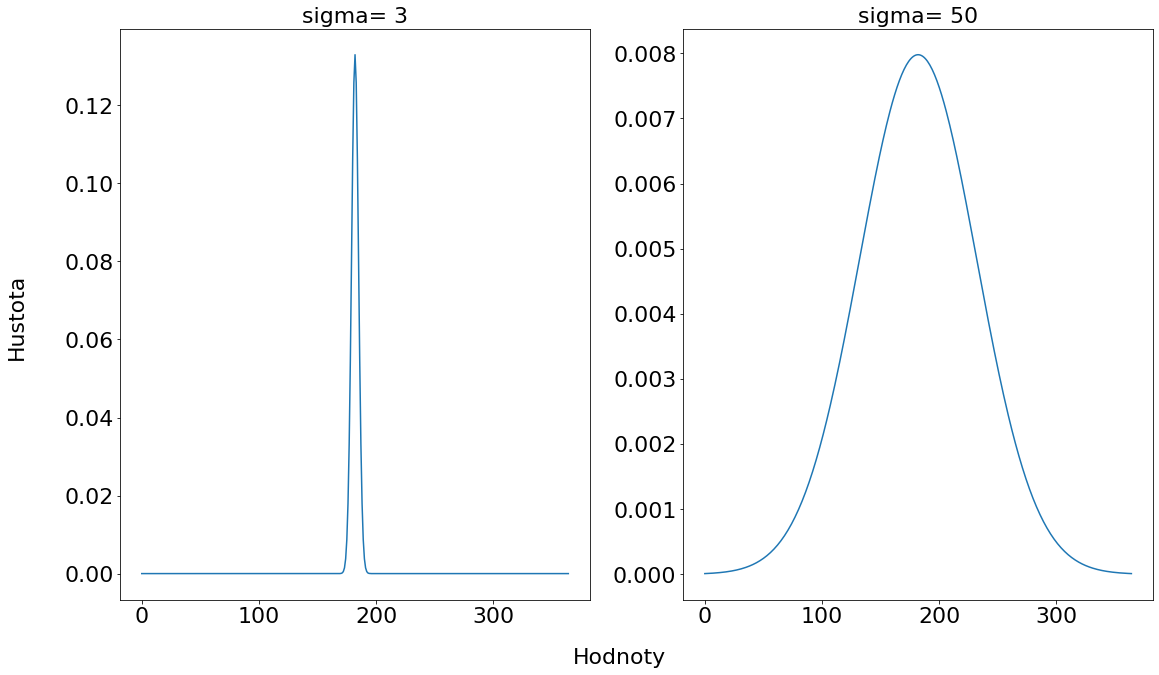
\includegraphics[width=\textwidth]{sigma.png}
\end{figure}

\subsection{Lokální extrémy}

Při průzkumu současných trendů v predikcích kryptoměn nás zaujal postup, který pro predikci volil lokální extrémy v posloupnosti Elliottových vln \cite{event-driven}. 
Tímto přístupem se autorům podařilo velice zredukovat problém predikce a dosahovali překvapivě dobrých výsledků. 
Proto jsme chtěli podobný přístup aplikovat na predikci kryptoměn. 
Pro predikci jsme nepoužívali teorii Elliottových vln.
Využili jsme ale pro predikci lokální extrémy z původního datasetu.

Pro nalezení lokálních extrémů jsme využili dataset s hodnotami kryptoměn a gaussův filtr, který je implementovaný v knihovně scipy jako \verb|scipy.ndimage.gaussian_filter1d|.
Hodnotu sigma jsme nastavili na 15, což nám zaručilo nalezení lokálních extrémů ve vyhlazeném grafu v rozmezí desítek minut.
Následně jsme nalezli lokální minima a maxima, která jsme umístili do dvou datasetů.
Poté jsme vytvořili zvlášť dvojice sousedních lokálních minim a maxim.
Mezi dvojicemi lokálních minim jsme v původním datasetu před použitím gaussova filtru hledali maximální hodnotu.
Stejný postup jsme provedli s dvojicí lokálních maxim a hledali jsme minimální hodnotu.
Výsledný dataset se poté skládal ze seřazené posloupnosti nalezených minimálních a~maximálních hodnot.
Tyto hodnoty tvořili skutečné lokální extrémy a tvořili základ výsledného datasetu.
Vzhledem k tomu, že skutečné lokální extrémy se hledají mezi lokálními extrémy vyhlazených dat, vyskytuje se poslední extrém příliš daleko od konce časové řady.
Tento problém jsme vyřešili umístěním posledního lokálního extrému mezi současný poslední lokální extrém a~konec dat.
Nalezení těchto extrémů je reprezentováno obrázkem \ref{visual:smooth}.
Dataset s předzpracovanými daty je pak tvořen hodnotami s časovým razítkem nalezených lokálních extrémů v datech s~kryptoměnami.

\begin{figure}
    \caption{Vyhlazení grafu a nalezení extrémů}
    \label{visual:smooth}
    \centering
    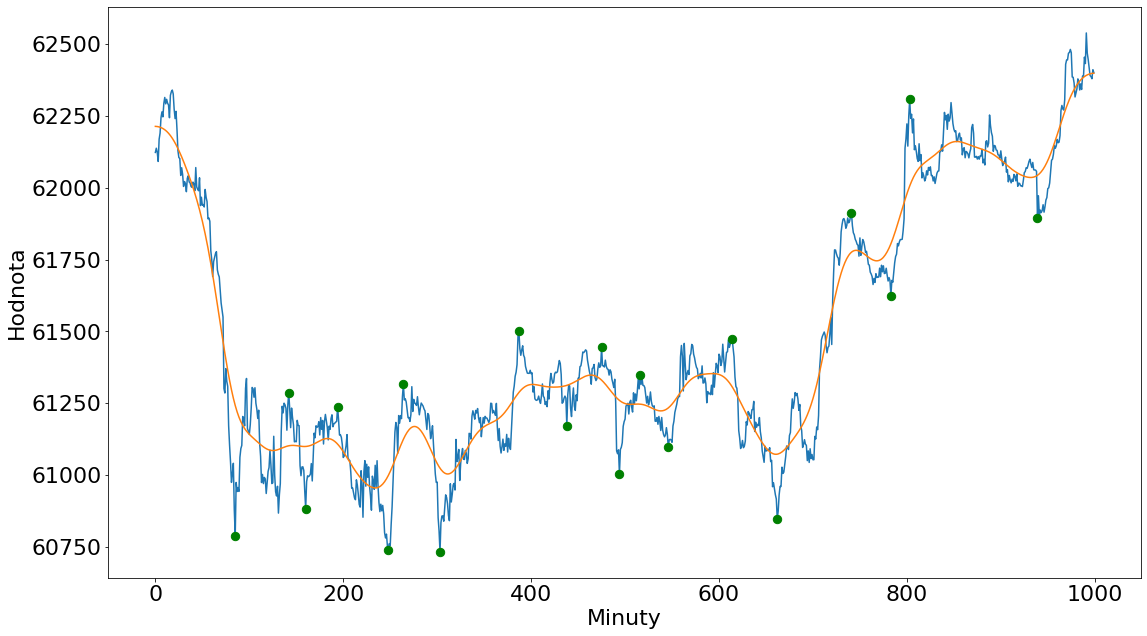
\includegraphics[width=\textwidth]{smooth.png}
\end{figure}

Dále výsledný dataset tvoří časová razítka jednotlivých extrémů s přesností na minuty. 
Z~původního datasetu jsou pak vytvářena vyhlazená data s použitím Gaussova filtru s hodnotou sigmy 15, 60 a 240. 
Z těch jsou vybírány body, ve kterých se vyskytují skutečné lokální extrémy z původního datasetu. 
Tento postup se třemi různými okny je prováděn pro data s hodnotami kryptoměn, data z Google Trends a pro data stažená z investing.com. 
Následně z nich stejným způsobem vybíráme body s časovým razítkem nalezených skutečných lokálních extrémů. 
U dat stažených z investing.com už však do výsledného datasetu zahrnujeme pouze vyhlazené hodnoty po aplikaci gaussova filtru a původní data již nepoužíváme. 
Tímto jsme vyřešili zkreslení dat z~této stránky před počátkem roku 2022, které máme uložené pouze s přesností na 5 minut.

\subsection{Stacionarita}

Časové řady jsou považovány za stacionární, pokud se jejich statistické vlastnosti, jako například momenty typu průměr nebo rozptyl, nemění v čase a zůstávají konstantní. 
Stacionarita zaručí, že každý bod je svojí hodnotou nezávislý na ostatních bodech v datasetu.
Toto neznamená, že všechny body v datasetu musí být stejné, ale figuruje zde garance zachování stejného chování vývoje hodnoty napříč celým datasetem. 
Při pohledu na graf stacionárních časových řad pak nebude možné pozorovat opakující se nebo dlouhodobý trend. 
Mnoho predikčních modelů zpracovávajících časové řady stacionaritu přímo vyžaduje. 
Jedná se například o řešení pomocí ARIMA modelu \cite{stationary:1, stationary:1}.

Způsobů pro ověření stacionarity existuje více. Nejzákladnější z nich je rozhodnutí na základě vizualizace. 
Pokud je možné po vytvoření grafu dat v čase pozorovat, že daty se šíří trend, nejedná se o~data stacionární. 
Dalším způsobem je využití autokorelační funkce. 
Ta porovnává data s~jejich zpožděnou kopií nazývanou lag. 
Takto je možné odhalit, jak velký lag je nutné zvolit pro snížení korelace dat. 
Pokud jsou zkoumaná data stacionární, hodnoty pro zvyšující se lag rychle konvergují k nulové hodnotě. 
Také můžeme využít ADF, rozšířený Dickey-Fullerův statistický test, který nám umožní prokázat hypotézu o pravděpodobnosti stacionarity. 
Tento test přesněji uvádí, do jaké míry může být naše hypotéza o stacionaritě zamítnuta. 
Pro samotné otestování hypotézy na našich datech jsme použili ADF s kódem \ref{adf} získaným v článku \uv{Why Does Stationarity Matter in Time Series Analysis} \cite{adf}. Pokud se na základě testu zamítne nulová hypotéza, znamená to, že časové řady nejsou stacionární. Testovali jsme 

\begin{lstlisting}[caption={~ADF},label=adf,captionpos=t,float,abovecaptionskip=-\medskipamount,belowcaptionskip=\medskipamount,language=Python]
from statsmodels.tsa.stattools import adfuller
def ADF_Cal(x):
    result = adfuller(x)
    ADF_stat = result[0]
    p = result[1]
    print("ADF Statistic: %f" % ADF_stat)
    print("p-value: %f" % p)
    print("Critical Values")
    levels = [.1, .05, .01]
    i = 0
    for key,value in result[4].items():
        print('\t%s: %.3f' % (key,value))
        hyp = p < levels[i]
        if ADF_stat < value:
            cert = (1-levels[i])*100
            print("{}% certain this is staionary".format(cert))
            print('Reject H0: {}'.format(hyp))
            break
        i = i+1
        if i >= 3:
            print("Less than 90% certain that data is stationary")
            print('Reject H0: {}'.format(hyp))
\end{lstlisting}

Data potřebujeme převádět do stacionárního stavu právě v důsledku jejich předešlé závislosti. 
Pokud vstup do našeho predikčního modelu tvoří nestacionární data, mohou se velice lišit přesnost predikovaných výsledků v závislosti na tom, kde se vstupní data nachází v původním datasetu. 
Nestálost přesnosti predikcí je tedy také jedním z ukazatelů stacionarity, protože k ní může docházet z toho důvodu, že zpracovaný úsek dat nereprezentuje korektně strukturu datasetu. 
U dat časových řas se však můžeme pokusit o řešení tohoto problému a převodu dat na stacionární s konstantní odchylkou a nulovou střední hodnotou. 

První a zároveň nejjednodušší metodou pro převod nestacionárních dat na stacionární je diferencování. 
Jedná se o odečtení dat od jejich předcházejících hodnot popsaných následující rovnicí:

\[\Delta y(t) = y(t) - y(t-1)\]

Konkrétně se jedná o diference první třídy. 
Těchto tříd můžeme využít neomezený počet pokud to naše potřeby vyžadují. 
Druhá třída od sebe odečítá sousední datové body, které byly výsledkem první diference. 
Jedná se o tento vzorec:

\[\Delta y(t) = y(t) - 2y(t-1) + y(t-2)\]

Ostatní třídy jsou od předchozích odvozeny stejným způsobem. 
Existuje také časové řady, které nelze převést na stacionární pomocí diferencování. 
Jedná se například o divergující časové řady, ve kterých se bude vyskytovat rostoucí nebo klesající trend po libovolném množství diferencování. 
Na tyto řady lze aplikovat logaritmickou transformaci, která data převede na podobu vhodnou pro diferencování \cite{stationary:2}.

Data s hodnotami kryptoměn máme v našem předzpracovaném datasetu v současné době zaznamenané pouze jako hodnoty v daných bodech. 
Tyto data stále disponují trendem a na základě testu ADF zamítáme tvrzení, že se jedná o stacionární data. 
Data získaná z Google Trends a investing.com se po předzpracování také jevila být nestacionární. 
Aplikovali jsme na ně tedy první třídu diferencí. 
Časové údaje, které jsme přidali do výsledného datasetu se však svojí strukturou liší od vývoje hodnot. 
Narozdíl od výše jmenovaných typů dat se tyto hodnoty vyvíjí pouze kladným směrem. 
Po provedení diference první třídy jsme převedli tyto údaje do podoby, kde reprezentují velikost časového okna mezi jednotlivými extrémy. 
Po dalším provedení diference jsme získali rozdíly jednotlivých časových oken. 
Nad těmito daty jsme tedy provedli diferenci druhé třídy \cite{stationary:3}.

\subsection{Výsledky po zpracování dat}

Rozšířený Dickey-Fullerův test prokázal, že data mohou být stacionární. 
To vyplývá i z vizuální kontroly datasetu kryptoměny Bitcoin na následujícím grafu. 
Konstrukce datasetu je vytvořena tak, aby bylo možné vytvářet jednoduše nové sloupce na základě nových dat, které chceme přidat do datasetu. 
Naším dalším krokem bylo vytvoření modelu, který bude na základě předchozích zpracovaných dat predikovat následující lokální extrém.

\section{Použité modely a jejich vrstvy}

\subsection{LSTM}

LSTM je typem rekurentních neboli opakujících se neuronových sítí. Zjednodušeně se jedná o~využití více neuronových sítí v rámci jednoho celku, díky kterému je pro síť možné zapamatovat si informace a využívat je dále v kombinaci s novými daty. 

Rekurentní neuronovou síť si lze představit, jako více kopií stejné sítě, z nichž každá předá data následující síti, která je na ní napojená. 
U samotných rekurentních neuronových sítí se ale vyskytuje problém s dlouhodobými závislostmi, nazývaný také problém mizejícího gradientu.
V~případě, že potřebujeme znát obsáhlý kontext dat je třeba využít vysokého množství provázaných neuronových sítí. 
Při učení se pak ale projeví právě mizející gradient.
Tedy situace, při které se učí pouze posledních pár neuronových sítí.
Z nalezení souvislosti mezi správným výsledkem rekurentní neuronové sítě a závislosti na velice dávném datovém údaji se stává téměř nemožný úkol.

Sítě s dlouhodobou krátkou pamětí, neboli LSTM jsou schopny odolat problému mizejícího gradientu a naučit se rozpoznávat i dlouhodobé závislosti.
Stejně, jako rekurentní neuronové sítě mají také strukturu podobnou řetězci, ale opakující se modul má komplexnější strukturu. V každém modulu se kombinují celkem 4 neuronové sítě \cite{lstm}. 
První v pořadí je síť využívaná pro odstraňování informací, která rozhoduje, zda se zachovají data z předchozího údaje.
Další je vstupní brána, která se používá pro kvantifikaci důležitosti nových informací na vstupu. 
Třetí síť tyto nové informace zpracovává a čtvrtou je výstupní brána, která vyhodnocuje celkový stav a poskytuje výstup \cite{gates}.

\subsection{Dropout a L2}

V práci využíváme nástroj pro tvorbu predikčních modelů Tensorflow. Ten nabízí množství nástrojů pro prevenci přeučení při trénování nového modelu. Nejpoužívanějšími z nich jsou metody Dropout a L2 regularizace. 

Vrstva Dropout je schopná náhodně vynulovat vybrané hodnoty vstupu během fáze trénování. To pak ve výsledku pomáhá zabránit přeučení. Ostatní hodnoty, které nejsou nastaveny na nulu jsou upraveny tak, aby se celkový součet všech vstupů nezměnil \cite{dropout}. 

Regularizace pomocí metody L2 pak zavádí penalizaci vah. Je schopná odstranit nízký počet vah a tím dosáhnout snížení rozdílu mezi testovací a trénovací chybou \cite{l2}.

\section{Predikce dat}

Dataset, který tvoří vstupní data do predikčního modelu byl vytvořen prostřednictvím metod pro předzpracování.
V případě dedikovaných modelů tvoří vstupy do jednotlivých modelů pouze vybrané sloupce tohoto datasetu.
Pro získání výsledných dat používáme alespoň 2 modely. 
Jsou využívány pro samostatnou predikci časového rozpětí mezi posledním lokálním extrémem a~nadcházejícím. 
Také predikujeme změnu hodnoty kryptoměny v následujícím lokálním extrému oproti minulé hodnotě. 
Jednotlivé kryptoměny obvykle následují ve stejném čase stejný trend. 
Mnoho z nich bylo totiž odvozeno od kryptoměny bitcoin nebo se s nimi často směna za bitcoin provádí \cite{btc-influence}.
To znamená, že jejich chování ve stejném časovém úseku je velice podobné. 
Byli jsme tedy schopní zkonstruovat jeden model pro predikci všech kryptoměn. 
Tento krok nám velice usnadnil a urychlil postupy při přidávání nových kryptoměn uživatelem. 
Nevyskytla se pak potřeba vytvářet nový model s každou novou kryptoměnou. 

Ačkoliv se ale některé kryptoměny vyvíjí podobně, mají jiné hodnoty. 
Tento problém jsme byli schopni vyřešit pomocí transformace hodnot na společné měřítko. 
Pro tento účel jsme využili knihovnu \verb|sklearn| a z ní nástroj na předzpracování \verb|PowerTransformer|. 
Ten se hlavně používá k tomu, aby distribuce dat přibližně odpovídala Gaussově distribuci. 
Využijeme přitom výchozí parametry. 
Na obrázku grafů hustoty hodnot \ref{transformation} můžeme vidět, že transformace opravdu převedla data na podobné hodnoty a je tedy opravdu možné použít pro jejich predikci stejný model.

\begin{figure}
    \caption{Hustota dat kryptoměn po transformaci}
    \label{transformation}
    \centering
    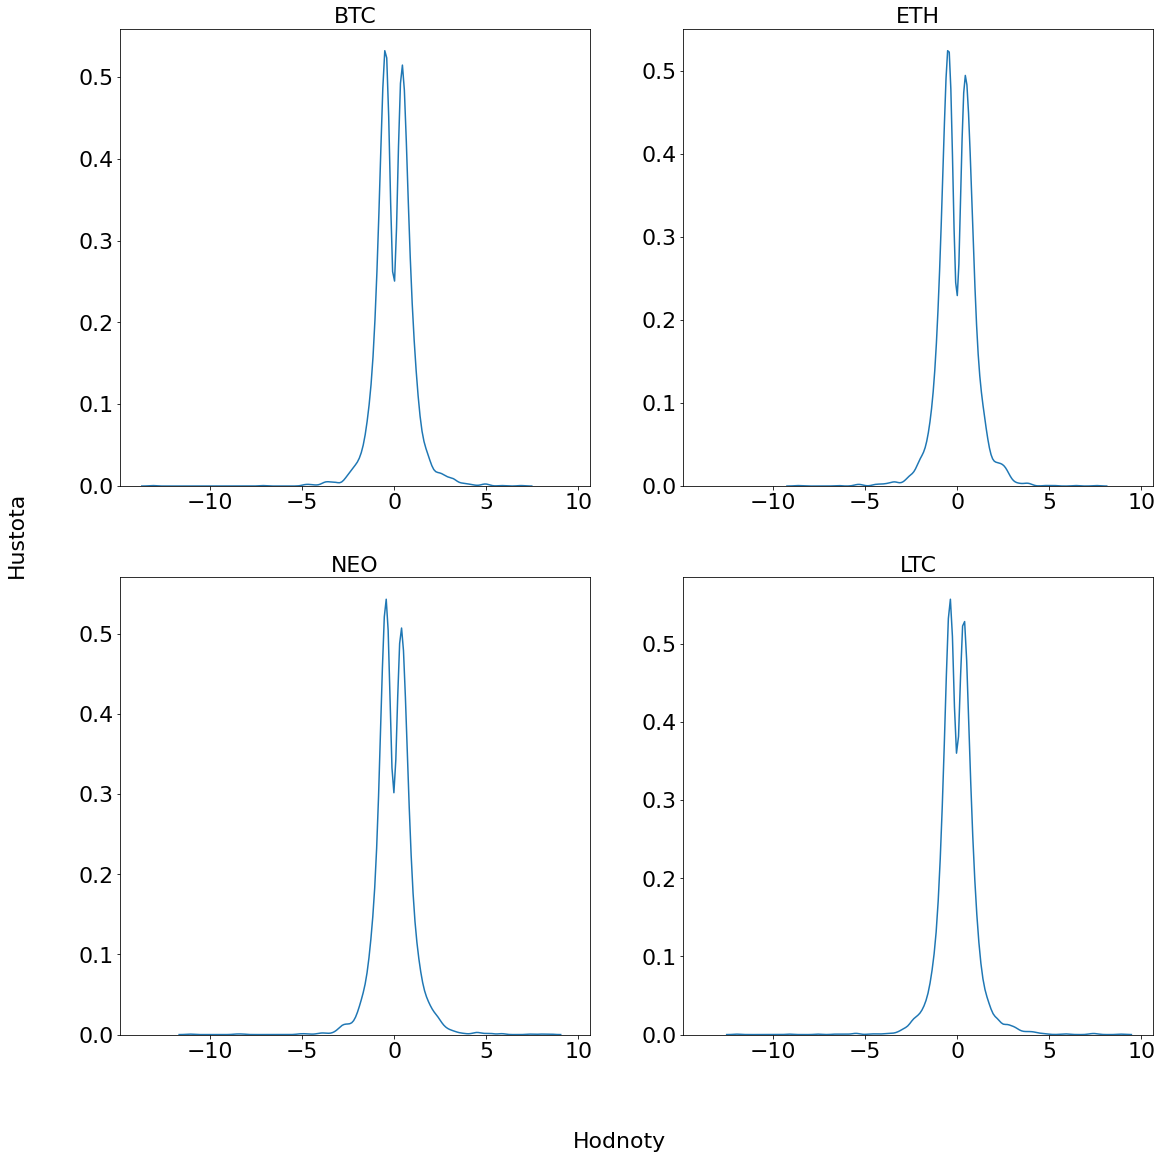
\includegraphics[width=\textwidth]{transformed.png}
\end{figure}

Ještě před tím, než jsme začali učit model na našich datech, bylo potřeba správně rozdělit data pro vylepšení odhadu přesnosti našeho modelu. 
Pokud by se například u našeho modelu projevilo přeučení, mohlo by se stát, že přesnost na datech určených k učení bude mít model vysokou na úkor přesnosti při predikci nových dat, která při učení použita nebyla. 
Z tohoto důvodu jsme rozdělili data na 3 části tak, jak za sebou data šla v čase.
Vzhledem k využívání paměťových bloků a predikce na základě posledních 50 údajů jsme takto získali testovací data, která žádným způsobem nezasahují do trénovacích. 
První část byla použita pro učení modelu.
Další pro určení chyby na datech, ke kterým model při učení neměl přístup a na základě kterých byly vybrány výsledné váhy modelu.
Poslední část dat dat byla využita pro určení výsledné přesnosti modelu s vybranými váhami. 
Dále bylo potřeba vybrat způsob měření chyby, které se model dopouští při predikcích. 
Pro měření predikce spojité hodnoty se nejčastěji používá průměrná absolutní odchylka MAE a průměrná kvadratická odchylka MSE popsané těmito vzorci:

\[MSE = \frac{1}{n}\sum (y-\hat{y})^2\]

\[MAE = \frac{1}{n}\sum |y-\hat{y}|\]

Z nich jsme vybrali MAE, protože dosahoval nižší výsledné průměrné absolutní chyby na testovacích datech.
Rozhodli jsme se pro sledování tohoto ukazatele, protože chceme hlavně snížit velikost celkového rozptylu chyb.

\subsection{Dedikované modely}

Jako první návrh jsme zkonstruovali model zobrazený v kódu \ref{first-model}. 
Ten následoval rozložení po vzoru projektu \uv{LSTM Neural Network for Time Series Prediction} \cite{predict-project} z repozitáře na serveru \url{github.com}.
Model byl autory používán pro predikci trendu v následujících časových bodech.
Tato predikce byla prováděna nad všemi daty z datasetu.
Na rozdíl od nich my však používáme lokální extrémy.
Při predikci s tímto modelem se projevilo přeučení.
Přesnost na trénovacích datech měřena pomocí průměrné absolutní chyby byla 0,002.
Chyba na validačních datech se ovšem ke konci trénování zvyšovala na hodnotu nad 1,0.
Proto bylo nutné zvolit jiný přístup k~predikci.

\begin{lstlisting}[caption={~1. model pro predikci},label=first-model,captionpos=t,float,abovecaptionskip=-\medskipamount,belowcaptionskip=\medskipamount,language=Python]
Model: "sequential"
_________________________________________________________________
Layer (type)                Output Shape              Param #   
=================================================================
lstm (LSTM)                 (None, 49, 256)           268288    

dropout (Dropout)           (None, 49, 256)           0         

lstm_1 (LSTM)               (None, 49, 256)           525312    

dropout_1 (Dropout)         (None, 49, 256)           0         

lstm_2 (LSTM)               (None, 49, 256)           525312    

dropout_2 (Dropout)         (None, 49, 256)           0         

lstm_3 (LSTM)               (None, 128)               197120    

dropout_3 (Dropout)         (None, 128)               0         

dense (Dense)               (None, 1)                 129       

=================================================================
Total params: 1,516,161
Trainable params: 1,516,161
Non-trainable params: 0
_________________________________________________________________
\end{lstlisting}

Tímto přístupem bylo vytvoření mnoha kompaktních modelů, z nichž každý by predikoval část dat. 
Ty byly rozděleny z původního předzpracovaného datasetu a jednotlivé modely zvlášť predikovaly následující lokální extrém kryptoměny například podle informací z Google Trends, S\&P 500 nebo ostatních monitorovaných ukazatelů. 
Tyto modely byly poté vrstvou v TensorFlow sloučeny do jednoho celku, který vracel jednu hodnotu, kterou mohlo být na základě vysvětlované proměnné interval nebo hodnota následujícího lokálního extrému. 
Každý z těchto modelů měl architekturu zobrazenou v kódu \ref{second-model}. 
Jejich úspěšnost se výrazně zlepšila a v průběhu tréninku nedocházelo k přeučení, čehož bylo dosaženo zavedením Dropout vrstvy a l2 regularizace. 
Výsledná hodnota MAE predikce pro časové intervaly byla 0,601 a pro hodnoty extrémů 0,328

\begin{lstlisting}[caption={~2. model pro predikci},label=second-model,captionpos=t,float,abovecaptionskip=-\medskipamount,belowcaptionskip=\medskipamount,language=Python]
Model: "sequential"
_________________________________________________________________
 Layer (type)                Output Shape              Param #   
=================================================================
 lstm (LSTM)                 (None, 49, 20)            2080      
                                                                 
 lstm_1 (LSTM)               (None, 4)                 400       
                                                                 
 dense (Dense)               (None, 1)                 5         
                                                                 
=================================================================
Total params: 2,485
Trainable params: 2,485
Non-trainable params: 0
_________________________________________________________________
\end{lstlisting}

\subsection{Společný model}

Při použití LSTM je možné aplikovat trénování ve směru dopředném i zpětném při použití obousměrné vrstvy, jak je to v této práci \uv{Cryptocurrency price prediction using LSTMs, TensorFlow for Hackers (Part III)} \cite{predict-model}.
Ta pro predikci hodnot využívá jeden kompaktní model s~LSTM obousměrnými vrstvami. 
Tento přístup jsme také otestovali a pomocí konstrukce modelu \ref{model:3} jsme dosáhli průměrné absolutní chyby intervalů 0,473 a 0,198 u hodnot extrémů. 
Toto řešení bylo dále méně časově náročné na trénování, a to až čtyřnásobně. 
Také se zlepšil čas predikce dat natrénovaným modelem vzhledem k jeho kompaktnosti. 
Model zároveň neprojevoval známky přeučení a jeho architektura tedy je využita ve finální verzi aplikace.

Po natrénování byly váhy tohoto modelu uloženy a v aplikaci jsou opět načteny po spuštění do nově vytvořeného modelu.
Trénování probíhalo v 5000 epochách a výsledný model dosahoval MAE 0.457 na časových predikcích a 0.162 na predikcích hodnoty dalšího extrému.

\begin{lstlisting}[caption={~Finální model pro predikci},label=model:3,captionpos=t,float,abovecaptionskip=-\medskipamount,belowcaptionskip=\medskipamount,language=Python]
    Model: "sequential"
_________________________________________________________________
 Layer (type)                Output Shape              Param #   
=================================================================
 bidirectional (Bidirectiona  (None, 49, 28)           3248      
 l)                                                              
                                                                 
 dropout (Dropout)           (None, 49, 28)            0         
                                                                 
 bidirectional_1 (Bidirectio  (None, 6)                768       
 nal)                                                            
                                                                 
 dropout_1 (Dropout)         (None, 6)                 0         
                                                                 
 dense (Dense)               (None, 1)                 7         
                                                                 
 activation (Activation)     (None, 1)                 0         
                                                                 
=================================================================
Total params: 4,023
Trainable params: 4,023
Non-trainable params: 0
_________________________________________________________________
\end{lstlisting}

Na tomto modelu jsme se rozhodli testovat, jaká data budeme k predikci využívat. 
V našem původním zpracovaném datasetu bylo celkem 9 nezávislých ukazatelů a další z nich odvozené.
Tento dataset jsme rozdělili na 7 částí. 
V každé z nich se vyskytovala data značící lokální extrémy kryptoměn a časové úseky. 
Dále se zde vyskytovaly jejich hodnoty v časech lokálních extrémů hodnot kryptoměn po vyhlazení Gaussovým filtrem.
Zbylá data byla v rámci jednotlivých datasetů vývoje hodnoty zlata, amerického dolaru, S\&P 500, VIX, NASDAQ a DJIA.
V tabulce \ref{results} je pak znázorněna průměrná absolutní chyba, které model dosahovat po trénování na jednotlivých datasetech.
Na základě těchto výsledků jsme se rozhodli, že celkový dataset bude obsahovat předzpracované údaje z dat o čase lokálních extrémů kryptoměn, jejich hodnotách, popularitě z~Google Trends a hodnotách zlata, S\&P 500 a VIX.

\begin{table}\centering
\caption{~Výsledky zkoumání vlivů různých dat na přesnost predikce}\label{results}
\begin{tabular}{l|c}
    Typ zkoumané hodnoty & Průměrná absolutní odchylka	\tabularnewline \hline 
     Zlato		    & 0,589	\tabularnewline \hline
     USD		    & 0,624	\tabularnewline \hline
     S\&P 500       & 0,573	\tabularnewline \hline
     VIX		    & 0,577	\tabularnewline \hline
     NASDAQ		    & 0,592	\tabularnewline \hline
     DJIA		    & 0,606	\tabularnewline \hline
     Google Trends	& 0,527	\tabularnewline 
\end{tabular}
\end{table}

\subsection{Genetický algoritmus}

Genetický algoritmus je vyhledávací heuristika, která je inspirována teorií přirozené evoluce publikované Charlesem Darwinem. 
V tomto algoritmu se odráží proces přírodního výběru, kdy jsou nejvýkonnější jedinci vybráni pro pokračování v evoluci. 
Tento proces začíná zavedením úvodního člena nebo členů, které tvoří první generaci populace. 
Následně se v rámci této generace provádí 2 typy operací. 
První z nich je křížení. 
Při tomto procesu se vyberou prvky z populace a~jejich vlastnosti se ve specifikovaném měřítku zkříží. 
Výsledkem je nový jedinec, který je následně přidán do populace. 
Dalším typem operace je mutace. 
Jedná se o proces, při němž se z jednoho člena populace vytvoří na základě předem specifikovaných parametrů člen nový \cite{genetic}.

Pro ohodnocení výkonu jedince je potřeba zavést fitness funkci, která bude určovat, jak si jedinec vede v porovnání s ostatními. 
Po otestování jedince mu bude uděleno touto fitness funkcí skóre určující pravděpodobnost, se kterou bude vybrán do nové generace.

Na základě predikcí našeho modelu jsme byli schopni určit, kdy nastane další lokální extrém a jaká bude jejich hodnota. 
Tyto predikce však nemusely být zcela přesné. 
Jejich nedostatek plynoucí z této nepřesnosti není možné nikdy zcela vyřešit a může se negativně podepsat na našem finančním zisku. 
Toto můžeme pozorovat na obrázku \ref{evolution} znázorňující výdělek náhodně vybrané kryptoměny v průběhu obchodování. 
Jeho hodnota znázorňuje poměr vůči původní částce a částce po ukončení dvojice operací nákup a prodej. 
Pro nákupy byly využity predikované údaje na základě zvolení rozhodnutí v kódu \ref{config}. 

\begin{figure}
    \caption{Vývoj zisku po jednotlivých transakcích}
    \label{evolution}
    \centering
    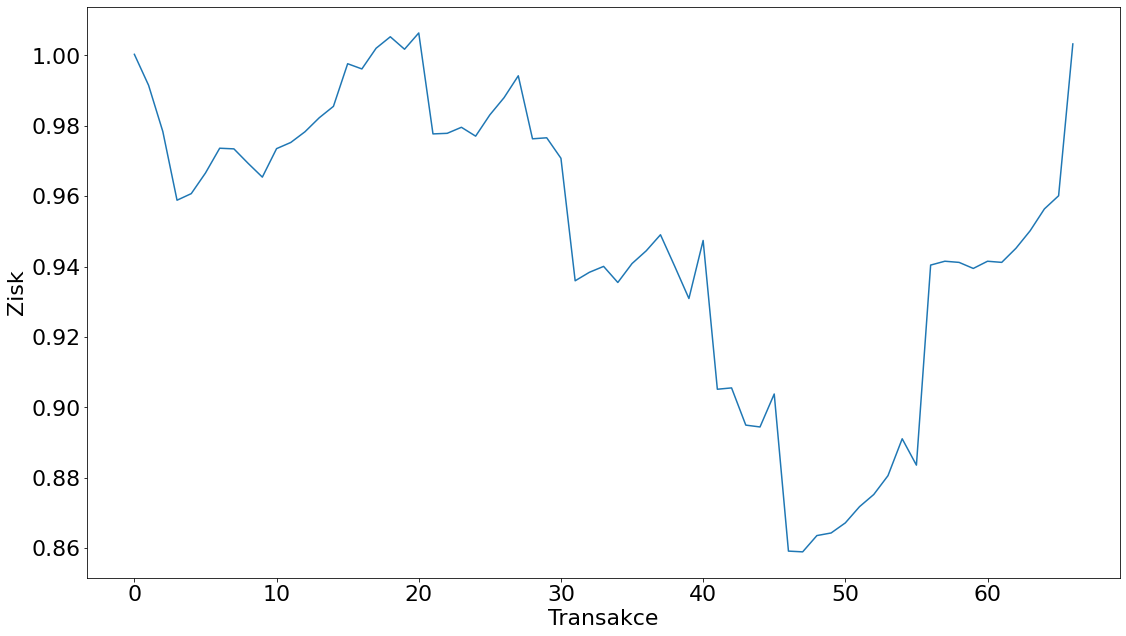
\includegraphics[width=\textwidth]{evolution.png}
\end{figure}

\begin{lstlisting}[caption={~Přiřazení akce na základě konfigurace},label=config,captionpos=t,float,abovecaptionskip=-\medskipamount,belowcaptionskip=\medskipamount,language=Python]
rising = config[0]
sinking = config[1]
time_buy_rising = config[2]
time_buy_sinking = config[3]
time_sell_rising = config[4]
time_sell_sinking = config[5]

advice = 'wait'

if growth > rising:
    if duration > time_buy_rising:
        advice = 'buy'
    if duration <= time_sell_rising:
        advice = 'sell'
if growth <= sinking:
    if duration < time_buy_sinking:
        advice = 'buy'
    if duration >= time_sell_sinking:
        advice = 'sell'
\end{lstlisting}

Pomocí genetického algoritmu jsme usilovali o nalezení takové konfigurace pro nakupování kryptoměn, při které uskutečněné nákupy v rámci obchodovacího období dosáhly kladného finančního zisku pro všechny kryptoměny. 
Náš genetický algoritmus byl pozměněn oproti své předepsané konstrukci vzhledem ke spojitým hodnotám jedinců populace. 
Struktura jedince je tvořena 6 hodnotami. Ten je pak použit v kódu \ref{config} pod názvem \verb|config|. 
Pomocí algoritmu se tedy hledají parametry prodeje a nákupu, díky kterým se aplikace může rozhodnout, kolik času musí uplynout po predikovaném lokálním minimu nebo kolik času musí zbývat u predikovaného lokálního maxima, aby mohla kryptoměny nakoupit. 
Prodej se pak řeší obdobným způsobem. 
Heuristická funkce, která určuje výkonnost jedinců vyhodnotí pro každou kryptoměnu zisk, kterého lze s danou konfigurací dosáhnout za zadané období. 
Z jednotlivých zisků kryptoměn se následně vybere nejnižší, kterého tato konfigurace dosáhla a toto číslo je vráceno jako její skóre. 
Nesnažíme se tedy maximalizovat celkový výdělek v rámci testovaných kryptoměn. 
Naším cílem je najít strategii, která nám umožní dosáhnout co nejlepšího výsledku napříč všemi kryptoměnami. 
Tímto se budeme snažit maximalizovat schopnost aplikace doporučovat výdělečnou strategii za každých okolností.

Data byla tvořena predikcemi z necelých 107 po sobě jdoucích dní. 
Pro predikce jsme využívali náš natrénovaný model a predikovali jsme následující lokální extrém v každé minutě našich dat. 
Celkem jsme tedy měli přibližně 107*24*60 predikcí seřazených v čase. 
Každá predikce se vztahovala k času poslední minuty, která byla zahrnuta v časovém okně dat tvořících vstupy pro predikci. 
Po každé predikci se posunulo toto časové okno o jednu minutu do budoucnosti. 

Toto řešení vedlo k pozitivnímu výsledku. Bylo nalezeno množství konfigurací, které maximalizovali minimální výdělek při obchodování s jednotlivými kryptoměnami. 
Následně bylo vizuálně porovnáno 25 nejvýdělečnějších konfigurací, pro výběr konečné konfigurace, která bude použita pro uskutečňování nákupu a která vykazovala dlouhodobě stoupající trend výdělku při jednotlivých transakcích. 
Jedná se o konfiguraci \verb|[0,69;-0,8;-96,7;57,43;281,61;15,63]|. 
V~této podobě umožní nákup, pokud je predikovaný růst trendu nad 0.69 a počet minut, do kdy má extrém podle predikce nastat je vyšší, než -96.7. 
Záporná hodnota je zde právě z důvodu jisté nepřesnosti při predikování časového údaje extrému a podle vyhodnocení genetického algoritmu je toto číslo ze zkoumaných konfigurací nejvýhodnější.
Graf, který zaznamenával výdělek při obchodování po každé transakci je znázorněn na obrázku \ref{best_config}.
Hodnota tohoto grafu je násobek původní hodnoty po provedení dvojice akcí nákupu a prodeje.
Celkově pak činil náš dosažený zisk téměř 40 \%. 

\begin{figure}
    \caption{Výdělek nejlepší vybrané konfigurace na 5 kryptoměnách}
    \label{best_config}
    \centering
    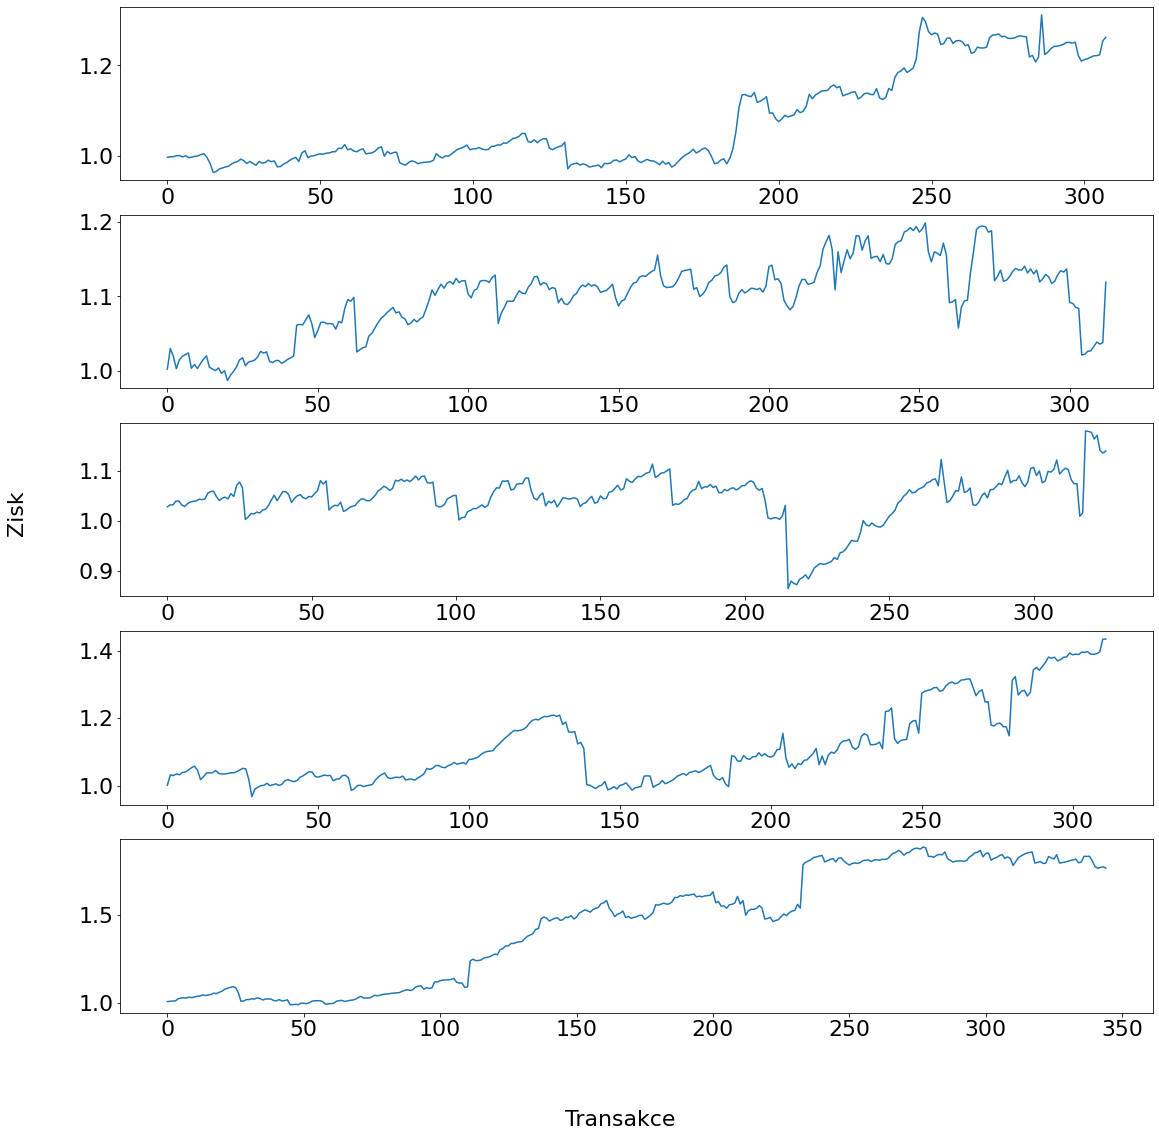
\includegraphics[width=\textwidth]{best_config.png}
\end{figure}

\chapter{Uživatelské rozhraní}

V této kapitole budeme konstruovat webové grafické uživatelské rozhraní. 
Budeme řešit rozložení grafických prvků, kaskádové styly, které použijeme, ale také komunikaci se serverem a optimalizaci přenosu dat.
Cílem našeho snažení má být přehledná grafická aplikace, která uživateli poskytne dostatečně podrobný přehled informací, aniž by působila dezorientačně.
Aplikace bude mít možnost zobrazovat jednotlivě i ve vyšším počtu grafy jednotlivých sledovaných ukazatelů.
Dále bude disponovat tabulkou, ve které budou zaznamenány predikce našeho natrénovaného modelu a rady uživateli, jak má na trhu s kryptoměnami postupovat na základě těchto predikcí.

\section{Frontend}

Pro zajištění orientace uživatele v naší aplikaci bylo třeba vytvořit grafické uživatelské rozhraní, které by poskytovalo přehled o vývoji veškerých sledovaných indexů, hodnot a ukazatelů. 
Soustředili jsme se na to, aby naše stránka poskytovala veškeré informace uživateli bez nutnosti přecházení mezi podstránkami a bez nutnosti scrollování. 
Tento přístup byl ale vzhledem k množství dat, kterými aplikace disponuje značně optimistický. 
Přesto jsme ale byli schopni co možná nejvíce omezit nutnost aktivní interakce uživatele s naším programem. 
Dále jsme se snažili poskytovat informace v takové podobě, aby uživateli přinesly co možná největší informační hodnotu a neznepřehledňovali přitom ostatní obsah na stránce. 
Výslednou podobu našeho uživatelského rozhraní je možné vidět na obrázcích \ref{visual:overview} a \ref{visual:table}.

\subsection{Vue.js}

Dynamická část grafického rozhraní byla konstruována pomocí Vue.js. 
Prostřednictvím tohoto rozhraní je pro uživatele generován graf, na kterém lze zobrazovat vývoj veškerých sledovaných indexů v reálném čase. 
Je zde také možnost přepnout se z přehledu všech sledovaných hodnot do zobrazení s predikcemi, kde může uživatel získat lepší přehled o predikovaném vývoji kryptoměn.
Dále Vue.js zobrazuje tabulku, ve které jsou zaneseny predikce budoucích lokálních extrémů a poslední lokální extrémy pro jednotlivé kryptoměny. 
Ve spodní části aplikace je tlačítko na přidání další sledované kryptoměny, po jehož kliknutí se uživateli zobrazí formulář pro zadání nové kryptoměny.

Graf, se uživateli zobrazuje v horní části aplikace. Zobrazuje ve výchozím režimu přehled událostí v reálném čase v rámci minut. 
Je tedy možnost v něm zobrazit například vyvíjející se hodnotu kryptoměn, jejich popularitu v rámci vyhledávání na Google Trends nebo hodnoty sledovaných komodit na investing.com. 
Hodnoty jednotlivých datasetů mají jiné měřítko. 
Cena Bitcoinu se pohybuje řádově v desítkách tisíc USD. 
Vyhledávání klíčových slov zase nabývá hodnoty mezi 0 a 100 a hodnota zlata se zase pohybuje v tisících. 
Oproti tomu DogeCoin má hodnotu desetin USD. 
Nedávalo by tedy smysl všechny tyto údaje uvádět v rámci jednoho společného měřítka. 
Místo toho jsme v grafu pro každý dataset vytvořili unikátní svislou osu, čímž bylo zaručeno, že veškerá zobrazená data mají maximální možnou viditelnost rozdílů mezi hodnotami jejich datových bodů v čase. 
Dále je takto možné snáze pozorovat závislosti mezi jednotlivými datasety. 
Například jsme schopni pozorovat závislost některých kryptoměn na vývoji hodnoty kryptoměny Bitcoin nebo vývoji kryptoměn na datech z Google Trends. 
Požadavek na nová data je zasílán každých 20 vteřin v rámci asynchronní funkce, ve které se dále čeká pomocí příkazu \verb|await| na odpověď serveru a následné zpracování dat. 

Tento přístup získávání dat ze serveru je označován jako promise-based HTTP klient. 
Promise neboli příslib označuje získání hodnoty, která nemusí být nutně známá při jeho vytvoření. 
Namísto okamžitého vrácení konečné hodnoty po volání se tedy vrátí jen jakási záruka, že data budou obdržena. 
Tento přístup nevylučuje neúspěch, nicméně řeší problém s čekáním na odpověď serveru. 
Nenastává tedy kolize mezi procesem získání dat a procesem pro jejich zpracování \cite{promise}.

Protože v grafu se zobrazují minutová data a funkce v našem frontendu odesílají požadavek a nová data každých 20 vteřin, bylo nutné optimalizovat náš kód. 
Při získávání dat z databáze se vrátí pouze dvojnásobek dat, který je následně zobrazen v grafu. Tato data jsou nadále zpracována, aby se v nich nevyskytovaly neplatné nulové hodnoty nebo chybějící hodnoty a veškeré datasety jsou zarovnány na stejný interval co nejblíže k současnosti.
Na rozdíl od ostatních dat nejsou data kryptoměn doplňována konstantní hodnotou mezi posledním časovým údajem a~současnou minutou. 
Ostatní datasety jsou však doplněna právě poslední zaznamenanou hodnotou.

Toto provedení umožňuje vytvoření komplexního způsobu aktualizace dat na vyžádání a jeho použití bylo popsáno v článku \uv{Getting Started with vue-chartjs} \cite{chart}.
Výslednou podobu našeho grafu je možné vidět na obrázku \ref{visual:overview}.

\begin{figure}
    \caption{Graf zobrazující vývoj hodnot sledovaných ukazatelů}
    \label{visual:overview}
    \centering
    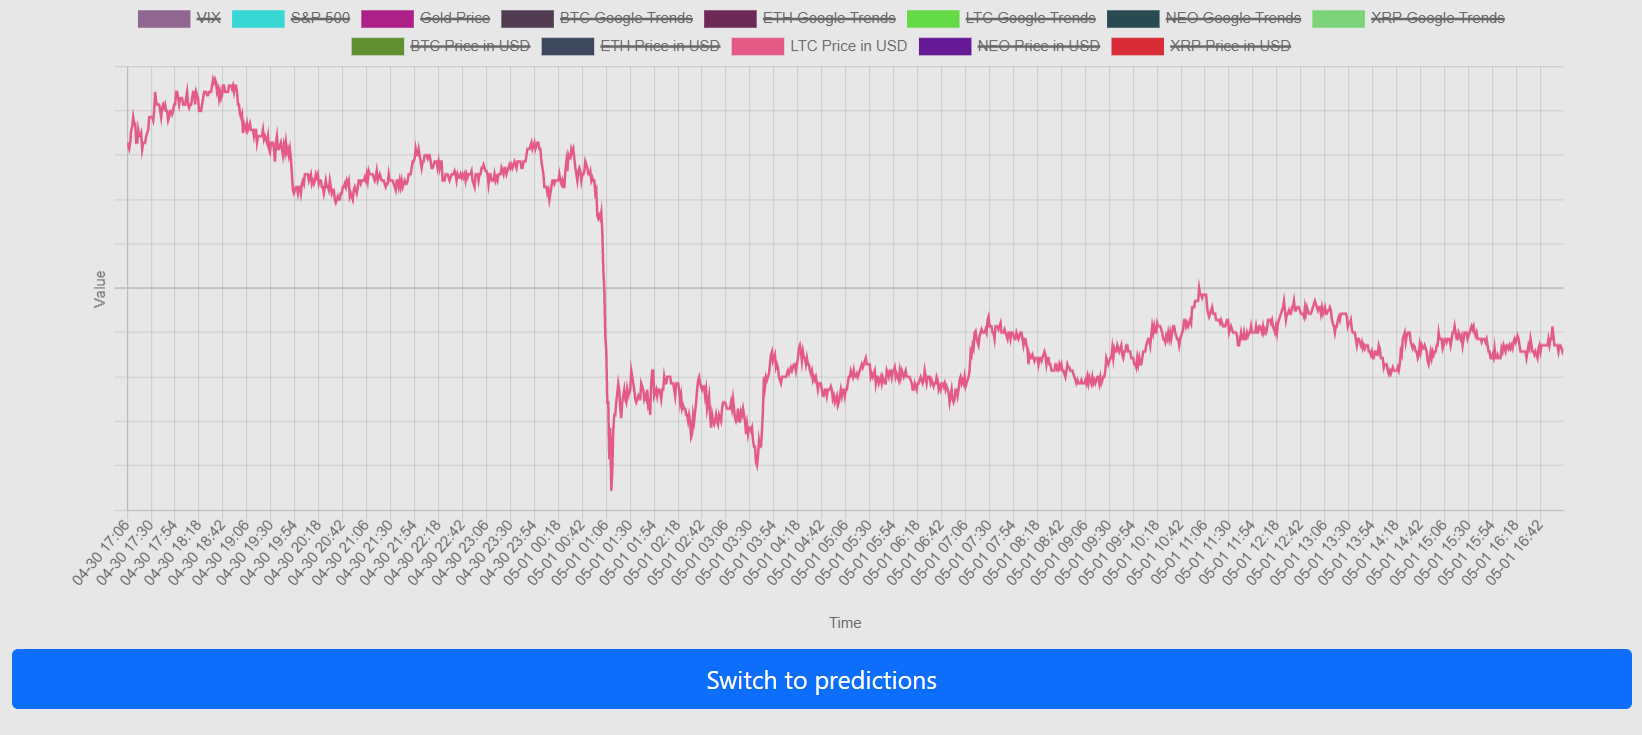
\includegraphics[width=\textwidth]{overview.png}
\end{figure}

Další typ grafu, který může uživatel zobrazit, obsahuje predikce. 
Je zde možné zobrazit na stejné ose jednak současný vývoj ceny kryptoměn, ale také poslední zaznamenaný lokální extrém a následující predikovaný extrém. 
Ty jsou spojeny přímkou. 
Přepínání mezi jednotlivými grafy je realizováno pomocí tlačítka ve spodní části oblasti grafu a při přepnutí si aplikace zapamatuje viditelnost jednotlivých dat, aby je pak po návratu k tomuto pohledu mohla zase stejným způsobem vykreslit.
Podoba predikcí je znázorněná na obrázku \ref{visual:predictions}.

\begin{figure}
    \caption{Graf zobrazující predikci hodnot sledovaných kryptoměn}
    \label{visual:predictions}
    \centering
    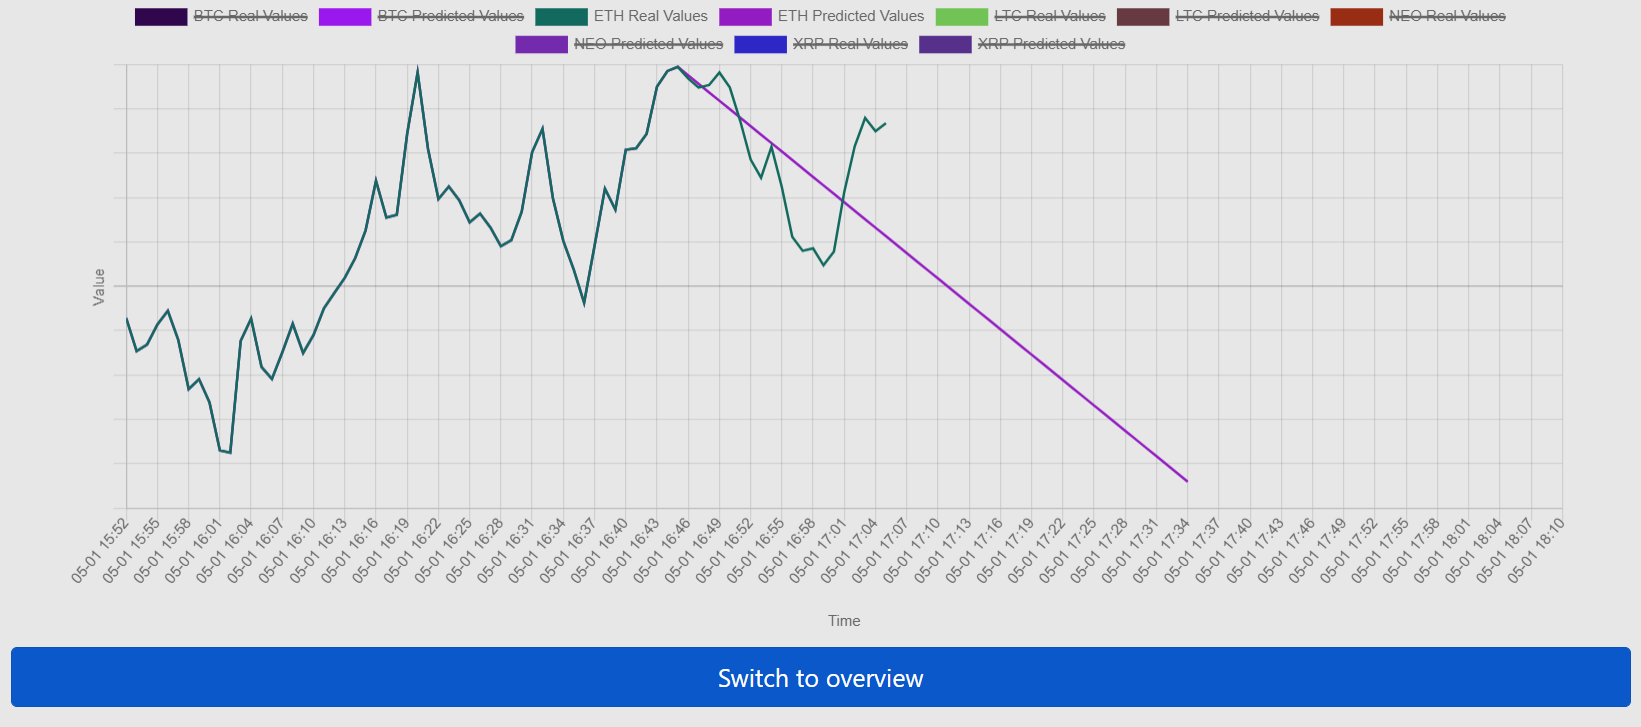
\includegraphics[width=\textwidth]{predictions.png}
\end{figure}

V dolní části aplikace se zobrazuje tabulka s přehledem. 
Je v ní zobrazen poslední zaznamenaný lokální extrém a predikovaný následující lokální extrém. 
Oba z nich jsou reprezentovány hodnotou a časem. 
V případě posledního zaznamenaného lokálního extrému se jedná o jeho přesný čas a hodnotu. 
V případě následujícího lokálního extrému je v tabulce zobrazena jeho predikovaná hodnota a čas, kdy by měl nastat. 
Dále se v tabulce vyskytuje jméno kryptoměn, pro které byly lokální extrémy zvoleny. 
Jména těchto kryptoměn lze do tabulky přidávat prostřednictvím tlačítka pro přidání kryptoměny vyskytujícího se pod tabulkou. 
Pokud si uživatel přeje některou evidovanou kryptoměnu odebrat, lze kliknout na ikonu odpadkového koše v tabulce. 
Po kliknutí na tuto ikonu se odešle dotaz na server s požadavkem odebrání této kryptoměny. 
V tabulce se pak její odebrání projeví okamžitě. V tabulce se dále zobrazuje vyhodnocení akce prostřednictvím konfigurace získané naším genetickým algoritmem. 
Na základě tohoto vyhodnocení se uživateli zobrazují doporučení akce z tabulky \ref{advice}. 
Dotaz na nová data tabulky se stejným způsobem jako u grafu odesílá obdobně každých 20 vteřin. 
\begin{table}\centering
\caption{~Doporučené akce pro maximalizaci zisku z obchodování s kryptoměnami}\label{advice}
\begin{tabular}{l|l}
    Doporučení & Význam	\tabularnewline \hline 
     Buy		    & Uživatel má okamžitě zakoupit kryptoměnu pro maximalizaci zisku	\tabularnewline \hline
     Wait		    & Uživatel nemá podnikat žádnou akci v důsledku vývoje hodnoty kryptoměny	\tabularnewline \hline
     Sell       	& Uživatel má okamžitě prodat kryptoměnu pro maximalizaci zisku	\tabularnewline 
\end{tabular}
\end{table}

Výslednou podobu naší tabulky je možné vidět na obrázku \ref{visual:table}.

\begin{figure}
    \caption{Tabulka s predikcemi a radami pro uživatele}
    \label{visual:table}
    \centering
    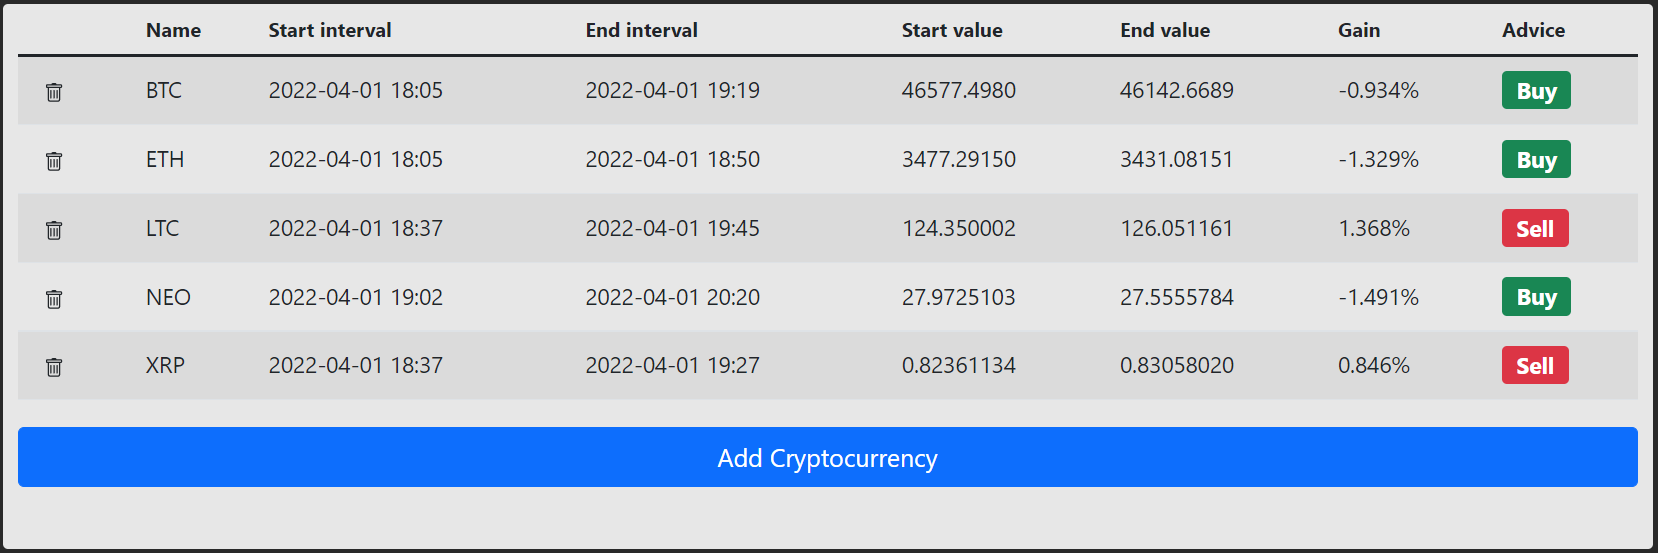
\includegraphics[width=\textwidth]{table.png}
\end{figure}

\subsection{CSS}

Pro docílení výsledného vzhledu uživatelského rozhraní bylo potřeba použít správných vizuálních prvků. 
K tomuto účelu jsme využili kaskádových stylů.
Ty reprezentují způsob úpravy vzhledu dokumentů napsaných v jazyce HTML. 
Popisují, jakým způsobem mají být prvky vykresleny na obrazovce. 
Umožňuje například změny barev a stylů písma, ale také zaoblení rohů nebo reaktivitu prvků po jejich interakci v podobě například změny barvy \cite{css}.

Pro úpravu vzhledu naší aplikace jsme použili předpřipravené kaskádové styly z frameworku bootstrap. 
Pod tímto názvem je označován open-source CSS framework zaměřený na responzivní frontend webový vývoj. 
My jsme konkrétně použili CSS specifikaci \url{https://cdn.jsdelivr.net/npm/bootstrap@5.1.3/dist/css/bootstrap.min.css} napříč celým projektem. 
To nám umožnilo získat a použít vzhled pro kontejnery tvořící pozadí prvků, tabulky, tlačítka text a~textová pole.

\subsection{HTML}

HTML je markup jazyk, s jehož pomocí můžeme definovat struktury obsahu naší webové aplikace. 
Právě prostřednictvím tohoto jazyka můžeme správně umístit do grafické části naší aplikace graf, tabulku a potřebné ovládací prvky. 
Každý z těchto prvků je vložen do kontejneru, který je tvořen strukturou div a od tmavého jednobarevného pozadí odděluje prvky v popředí. 
Samotný kontejner, na kterém se naše grafické prvky nachází má světlou barvu a zaoblené rohy. 
Jednotlivé kontejnery od sebe dále odděleny viditelným paddingem. 
Tento vzhled jednak logicky odděluje grafické prvky a zároveň na uživatele působí moderně a přívětivě. 
V tabulce je definovaný \verb|v-for| cyklus, díky kterému můžeme pomocí Vue.js aktualizovat hodnoty v ní. 
Posledním prvkem v~HTML dokumentu, který specifikuje rozklad našich prvků je formulář na přidání nových kryptoměn. 
Ten se zobrazí pouze ve chvíli, kdy uživatel klikne na tlačítko přidání. 
Možnost skrýt prvky a zobrazit je pouze po akci uživatele nám poskytuje BootStrap CSS knihovna. 
Pro využití této schopnosti stačí pouze nastavit třídu kontejneru mizícího prvku jako \verb|modal fade| a specifikovat jeho id v tlačítku pro jeho zviditelnění \cite{bootstrap}.

\section{Backend}

Pokud chceme používat Flask framework, musíme napřed vytvořit instanci naší webové aplikace. 
Následně se tato aplikace spustí příkazem "run", v rámci kterého se také specifikuje adresa, na které má být webové rozhraní přístupné. 
Tímto způsobem budeme ve výsledku schopni zobrazit naší aplikaci na adrese \url{http://localhost} a výchozím portu 5000. 
Máme také možnost prostřednictvím tohoto frameworku zobrazovat naší webovou aplikaci.
Musíme ale napřed specifikovat, jakým způsobem k ní chceme přistupovat. 
K tomuto účelu slouží dekorátory, v rámci kterých jsme definovali cestu k jednotlivým částem aplikace. 

Kromě načítání a vykreslování souborů s HTML strukturou můžeme také stejným způsobem přistupovat k dynamickým prvkům v jazyce JavaScript a kaskádovým stylům.
Flask disponuje metodou \verb|render_template|, která nám právě tento přístup umožnila. 
Její použití včetně dekorátoru je v kódu \ref{render}.

\begin{lstlisting}[caption={~Vykreslování šablony},label=render,captionpos=t,float,abovecaptionskip=-\medskipamount,belowcaptionskip=\medskipamount,language=Python]
@app.route('/')
def get_view():
    return render_template('index.html')    
\end{lstlisting}

Specifikovali jsme zde cestu \verb|'/'|.
Tato cesta specifikuje strukturu za zadanou adresou serveru a portu.
Plnohodnotná adresa má tedy tvar \url{http://localhost:5000/}. 
Soubory s kódem pro frontend musí být umístěny v přesně specifikované adresářové struktuře, kterou Flask framework respektuje. 
Tu jsme vytvořili následovně:

\dirtree{%
    .1 .
    .2 static.
    .3 js.
    .4 chart.js.
    .4 table.js.
    .3 styles.
    .4 styles.css.
    .2 templates.
    .3 index.html.
}

\

Soubory \verb|chart.js| a \verb|table.js| obsahují kód pro dynamické vykreslování grafu a tabulky společně se získáváním jejich dat ze serveru.
Soubor \verb|styles.css| obsahuje kaskádové styly pro grafické prvky aplikace a soubor \verb|index.html| obsahuje statické rozložení prvků naší aplikace.

Obdobně, jako funkci pro vykreslení stránky jsme také definovali funkce, které komunikují s frontendem. 
Jejich návratové hodnoty jsou ovšem předzpracovaná data ve formátu \textit{JSON}. 
Veškeré používané cesty z kořenové adresy jsou specifikovány v tabulce \ref{paths}.
Součástí serverové části aplikace, která převádí data do podoby pro zobrazení v grafu je i simulace nakupování a~prodávání kryptoměn na základě vyhodnocených doporučení akcí pro uživatele. V případě, že nejlepší vyhodnocená akce je nákup, zaznamená se do databáze tato akce se současnou hodnotou specifikované kryptoměny. V případě prodání se vypočte výnos, který by transakce potencionálně zaručila. Informace o současné hodnotě kryptoměn jsou získávány z API \url{binance.com}.

\begin{table}\centering
    \caption{~Cesty z kořenové webové adresy}\label{paths}
    \begin{tabular}{l|l|l}
        Typ požadavku & Adresa & Popis	\tabularnewline \hline 
        POST & /add/		    & Přidání kryptoměny do aplikace	\tabularnewline \hline
        POST & /remove/       & Odebrání kryptoměny z aplikace	\tabularnewline \hline
        GET & /data/		    & Data pro konstrukci nebo aktualizaci tabulky s predikcemi	\tabularnewline \hline
        GET &  /chart/	    & Data potřebná pro konstrukci a aktualizaci grafu	\tabularnewline
    \end{tabular}
\end{table}

\chapter{Architektura a vývoj aplikace}

\section{Oddělení kontejnerů}

Po naší aplikaci jsme vyžadovali, aby byla odolná vůči případným selháním jejích dílčích částí. 
Také jsme chtěli mít možnost během jejího chodu nasazovat nové podpůrné funkce a řešení. 
Z~tohoto důvodu jsme si pro běh zvolili kontejnerovou strukturu, která je zprostředkována platformou Docker. 
Jednotlivé části jsou schopny fungovat jako samostatný celek a je tedy potřeba je vhodně využívat v rámci jedné aplikace. 
Důležité bylo zařídit mezi těmito samostatnými aplikacemi a~databází komunikaci, v rámci které probíhá jejich interakce. 

Konfiguraci databáze PostgreSQL jsme specifikovali v souboru docker-compose.yml, který se v příkazu k sestavení \verb|docker-compose -f .devcontainer/docker-compose.yml up -d| předá jako parametr. 
Tímto jsme vytvořili funkční databázi viditelnou a přístupnou pouze ostatními kontejnery definovanými v souboru. 
Pomocí parametru \verb|restart: unless-stopped| jsme zajistili, že pokud by nastala situace, při které by se vypnul image nebo počítač, pak se kontejner s touto částí aplikace automaticky restartuje. 
Tento parametr zavedeme u všech kontejnerů. 

Ostatní části aplikace nemají definovanou konfiguraci jejich image přímo v konfiguračním souboru docker-compose.yml. 
Nachází se ve svých dedikovaných složkách. 
Protože se kód všech částí aplikace až na databázi spouští v programovacím jazyce Python, má jejich image \verb|python:3.8| již předpřipravené prostředí pro tento programovací jazyk. 
Jedná se o verzi tohoto programovacího jazyka, kterou podporují veškeré použité nástroje a která je stále v aktivní podpoře a~údržbě. 
Konfigurace jsou v rámci svých dedikovaných složek specifikovány v souborech Dockerfile a společně s nimi se ve stejném adresáři vyskytují specifikované moduly, knihovny a balíčky vyžadované kódem spouštěným daným kontejnerem. 
Ty se po prvním spuštění kontejneru automaticky nainstalují.
Kontejner pro stahování dat z Google Trends tedy má v požadavcích na python specifikovanou mimo jiné knihovnu requests pro zasílání požadavků. 
Dockerfile pro kontejner stahující data ze stránky \url{investing.com} navíc oproti ostatním obsahuje instalaci aplikací chromium a chromium-driver, které mu umožní přístup na internet prostřednictvím nástroje Selenium. 
Na konci každé specifikace kontejneru je blokující příkaz, který zapne dílčí program. 

Připojení k databázi z kontejnerů probíhá podobným způsobem, jako při přístupu mimo ně. 
Knihovna psycopg2 poskytuje rozhraní pro připojení a komunikaci. 
Při pokusu o připojení se specifikuje uživatel, heslo, host, port a databáze. 
Pokud bychom přistupovali mimo kontejner, nastavili bychom adresu hostu na adresu databáze. 
Zde je místo adresy specifikované jméno kontejneru, ve kterém se databáze nachází. 
Docker sám tuto závislost vyřeší a dosadí za jméno kontejneru adresu databáze. 

\newpage

Pro možnost přistupovat a zobrazovat grafické uživatelské rozhraní mimo oddělené prostředí kontejnerů bylo potřeba napřed specifikovat porty, které byly vystaveny pro vnější komunikaci. 
Tím jsme dosáhli, že se adresa, na které mělo být webové rozhraní přístupné, přepsala na \verb|0.0.0.0|. 
Tímto způsobem se adresa naší aplikace veřejně vystavila v rámci sítě, na které se naše zařízení vyskytuje. 
To v praxi znamená, že naše aplikace je přístupná i mimo síť kontejneru na zařízení, které docker knontejnery a tedy i naší aplikaci hostuje.

\chapter{Závěr}

Cílem této práce byla konstrukce webové aplikace, která by zobrazovala uživatelům přehled o~kryptoměnách. 
Tento přehled zahrnoval také predikce vývoje hodnot cen, pro které byl vytvořen predikční model. 
Vstup do tohoto modelu byla předzpracovaná data stažená z internetů pomocí zkonstruovaných scraperů.

V první části práce jsme analyzovali současné metody používané při predikci a obchodování na finančních burzách.
Rozhodli jsme se, že na základě jednoho z přístupů použijeme predikci následujících lokálních extrémů.
Napřed jsme zkonstruovali nástroje pro stahování dat z internetu. 
Stahovali jsme data o vývoji hodnot kryptoměn, příspěvky ze sociální sitě Twitter, data o~počtu vyhledávání z Google Trends a více různých indexů ze serveru \url{investing.com}.
Některé zdroje disponovaly pouze nízkou ochranou proti strojovému přístupu k datům a bylo možné je získat prostřednictvím odeslání HTTP požadavků.
K jiným, jako například k datům ze stránky \url{investing.com}, byl již obtížnější přístup a bylo potřeba využít nástroje Selenium ke stažení dat.
Zjistili jsme, že je výpočetně neúnosné zařadit do výpočtů výsledky ze sociální sítě Twitter.
Nebyl to pro nás ale problém, protože na základě analyzovaných prací a přístupů vyšlo jako mnohem výhodnější použít data o vyhledávání na vyhledávacím enginu Google.

Dále jsme se zabývali předzpracováním dat. 
Všechna data jsme se snažili převést na stacionární pro zvýšení přesnosti následné predikce.
Pro predikci jsme chtěli použít jednotný model, a tedy jsme potřebovali hodnoty dat převést na stejné měřítko. 
Toho jsme dosáhli použitím transformace převádějící data do podoby gaussovy křivky.
Výsledný dataset s předzpracovanými daty byl tvořen vybranými body v časech lokálních extrémů kryptoměn.

Při tvorbě modelu jsme napřed zkoušeli přístupy popsané ve vysoce hodnocených projektech z repozitáře gitlab.com.
Tento model ovšem při použití našich dat trpěl přeučením a bylo nutné vytvořit vlastní.
Následně jsme tedy zkoušeli dedikované modely pro části z původního datasetu s~předzpracovanými daty.
Dosáhli jsme celkového zlepšení a zamezili jsme přeučení.
Jako poslední model jsme použili obousměrné vrstvy LSTM bloků v rámci jednoho jednoduchého modelu, který predikoval výsledky na základě všech dat z předzpracovaného datasetu.
Tento přístup se ukázal jako nejpřesnější, a tedy byl implementován v konečné verzi aplikace.
Ze stahovaných indexů ze serveru investing.com byly nakonec vybrány pouze cena zlata, hodnota S\&P 500 a VIX, protože bylo vyhodnoceno, že přináší významné zlepšení přesnosti predikce.

Následně jsme se na základě predikcí snažili vyhodnotit strategii, která by maximalizovala náš výdělek při obchodování.
K tomuto účelu jsme využili genetický algoritmus.
Takto jsme nalezli ideální hladinu růstu hodnoty, která je vhodná k nákupu nebo hladinu poklesu k prodeji.
Tímto přístupem jsme získali konfiguraci o 6 ukazatelích, které určují, zda má uživatel koupit kryptoměnu, prodat jí nebo čekat na změnu současného chování hodnoty kryptoměny.

Poslední samostatnou částí naší aplikace byl frontend. 
Ten poskytuje uživateli přehled o~kryptoměnách.
Pro vývoj dynamické části, která se stará o obnovu dat na obrazovce, jsme použili Vue.js.
Tento framework je také schopný zasílat HTTP dotazy, což je způsob, jakým jsme získávání dat implementovali.
Pro backend aplikace pro komunikaci a zpracování dat před odesláním je využit nástroj Flask, díky němuž jsme schopní otevřít aplikaci na specifikované adrese \url{http://localhost:5000}.

Použití nástroje Selenium pro stahování dat z \url{investing.com} bylo nutné až v průběhu vývoje, kdy poskytovatel dat změnil své rozhraní. 
Z tohoto poznatku lze tedy usoudit, že do budoucna tento problém může nastat znovu. 
V takovém případě bude nutné upravit scraper příslušných dat, aby bylo možné data dále získávat.
Během testování bylo zjištěno, že po zvýšení počtu dotazů na datové servery v rámci minut dojde k zablokování přístupu naší aplikace k těmto datům.
Nejednalo se o vážný problém, protože současná perioda stahování dat byla dostatečná. 
Přesto jsme se ale pokoušeli tento nedostatek odstranit. 
Bylo zjištěno, že při použití VPN a automatické změně serveru každých 15 minut můžeme na datové servery zasílat vysoké množství dotazů.

Aplikace, která je výsledkem této práce je schopná doporučovat uživateli, jaké akce podniknout pro dosažení výdělku při obchodování s kryptoměnami.
V rámci testování byl zkoumán nákup celkem 5 kryptoměn po dobu 3 měsíců a s použitím konfigurace nalezenou pomocí genetického algoritmu bylo dosaženo kladného výdělku u všech z nich.
Do budoucna by šla tato práce rozšířit o automatické obchodování bez nutnosti zapojování uživatele.
Tento proces by eliminoval zpoždění mezi poskytnutím rady uživateli a jeho akcí.
Zároveň se takto odstraní i možnost zásahu uživatele do transakce, kterou by mohl ohodnotit, jako nevhodnou.
Proto je toto řešení ponecháno pouze jako návrh. % include `text.tex' from `text/' subdirectory

\appendix\appendixinit % do not remove these two commands

%\chapter{Nějaká příloha}


Sem přijde to, co nepatří do hlavní části.
 % include `appendix.tex' from `text/' subdirectory

\backmatter % do not remove this command

\printbibliography % print out the BibLaTeX-generated bibliography list

\chapter{Obsah přiloženého média}


	\dirtree{%
		.1 readme.txt\DTcomment{stručný popis obsahu média a návod k administraci a spuštění aplikace}.
		.1 .devcontainer\DTcomment{konfigurační soubory pro jednotlivé kontejnery aplikace}.
		.1 app\DTcomment{vlastní kód aplikace}.
		.2 ai\DTcomment{nástroje pro administraci umělé inteligence a predikcí}.
		.2 scraper\DTcomment{nástroje pro stahování dat z internetu}.
		.2 ui\DTcomment{nástroje pro stahování dat z internetu}.
		.2 utils\DTcomment{nástroje pro hlášení stavu a správu uložiště}.
		.1 data\DTcomment{zálohovaná data z databáze s konfiguracemi vytvořenými metodami z adresáře \texttt{ai}}.
		.1 saved\_model\DTcomment{uložené váhy natrénovaných predikčních modelů}.
		.1 text\DTcomment{text práce}.
		.2 thesis.pdf\DTcomment{text práce ve formátu PDF}.
		.2 src\DTcomment{zdrojový kód textu práce}.
	}
 % include `medium.tex' from `text/' subdirectory

\end{document}
